% Options for packages loaded elsewhere
\PassOptionsToPackage{unicode}{hyperref}
\PassOptionsToPackage{hyphens}{url}
%
\documentclass[
  Letterpaper,
]{scrbook}

\usepackage{amsmath,amssymb}
\usepackage{iftex}
\ifPDFTeX
  \usepackage[T1]{fontenc}
  \usepackage[utf8]{inputenc}
  \usepackage{textcomp} % provide euro and other symbols
\else % if luatex or xetex
  \usepackage{unicode-math}
  \defaultfontfeatures{Scale=MatchLowercase}
  \defaultfontfeatures[\rmfamily]{Ligatures=TeX,Scale=1}
\fi
\usepackage{lmodern}
\ifPDFTeX\else  
    % xetex/luatex font selection
    \setmainfont[]{Noto Serif CJK SC}
\fi
% Use upquote if available, for straight quotes in verbatim environments
\IfFileExists{upquote.sty}{\usepackage{upquote}}{}
\IfFileExists{microtype.sty}{% use microtype if available
  \usepackage[]{microtype}
  \UseMicrotypeSet[protrusion]{basicmath} % disable protrusion for tt fonts
}{}
\makeatletter
\@ifundefined{KOMAClassName}{% if non-KOMA class
  \IfFileExists{parskip.sty}{%
    \usepackage{parskip}
  }{% else
    \setlength{\parindent}{0pt}
    \setlength{\parskip}{6pt plus 2pt minus 1pt}}
}{% if KOMA class
  \KOMAoptions{parskip=half}}
\makeatother
\usepackage{xcolor}
\usepackage[paperwidth=6in,paperheight=9in]{geometry}
\setlength{\emergencystretch}{3em} % prevent overfull lines
\setcounter{secnumdepth}{5}
% Make \paragraph and \subparagraph free-standing
\makeatletter
\ifx\paragraph\undefined\else
  \let\oldparagraph\paragraph
  \renewcommand{\paragraph}{
    \@ifstar
      \xxxParagraphStar
      \xxxParagraphNoStar
  }
  \newcommand{\xxxParagraphStar}[1]{\oldparagraph*{#1}\mbox{}}
  \newcommand{\xxxParagraphNoStar}[1]{\oldparagraph{#1}\mbox{}}
\fi
\ifx\subparagraph\undefined\else
  \let\oldsubparagraph\subparagraph
  \renewcommand{\subparagraph}{
    \@ifstar
      \xxxSubParagraphStar
      \xxxSubParagraphNoStar
  }
  \newcommand{\xxxSubParagraphStar}[1]{\oldsubparagraph*{#1}\mbox{}}
  \newcommand{\xxxSubParagraphNoStar}[1]{\oldsubparagraph{#1}\mbox{}}
\fi
\makeatother


\providecommand{\tightlist}{%
  \setlength{\itemsep}{0pt}\setlength{\parskip}{0pt}}\usepackage{longtable,booktabs,array}
\usepackage{calc} % for calculating minipage widths
% Correct order of tables after \paragraph or \subparagraph
\usepackage{etoolbox}
\makeatletter
\patchcmd\longtable{\par}{\if@noskipsec\mbox{}\fi\par}{}{}
\makeatother
% Allow footnotes in longtable head/foot
\IfFileExists{footnotehyper.sty}{\usepackage{footnotehyper}}{\usepackage{footnote}}
\makesavenoteenv{longtable}
\usepackage{graphicx}
\makeatletter
\newsavebox\pandoc@box
\newcommand*\pandocbounded[1]{% scales image to fit in text height/width
  \sbox\pandoc@box{#1}%
  \Gscale@div\@tempa{\textheight}{\dimexpr\ht\pandoc@box+\dp\pandoc@box\relax}%
  \Gscale@div\@tempb{\linewidth}{\wd\pandoc@box}%
  \ifdim\@tempb\p@<\@tempa\p@\let\@tempa\@tempb\fi% select the smaller of both
  \ifdim\@tempa\p@<\p@\scalebox{\@tempa}{\usebox\pandoc@box}%
  \else\usebox{\pandoc@box}%
  \fi%
}
% Set default figure placement to htbp
\def\fps@figure{htbp}
\makeatother
% definitions for citeproc citations
\NewDocumentCommand\citeproctext{}{}
\NewDocumentCommand\citeproc{mm}{%
  \begingroup\def\citeproctext{#2}\cite{#1}\endgroup}
\makeatletter
 % allow citations to break across lines
 \let\@cite@ofmt\@firstofone
 % avoid brackets around text for \cite:
 \def\@biblabel#1{}
 \def\@cite#1#2{{#1\if@tempswa , #2\fi}}
\makeatother
\newlength{\cslhangindent}
\setlength{\cslhangindent}{1.5em}
\newlength{\csllabelwidth}
\setlength{\csllabelwidth}{3em}
\newenvironment{CSLReferences}[2] % #1 hanging-indent, #2 entry-spacing
 {\begin{list}{}{%
  \setlength{\itemindent}{0pt}
  \setlength{\leftmargin}{0pt}
  \setlength{\parsep}{0pt}
  % turn on hanging indent if param 1 is 1
  \ifodd #1
   \setlength{\leftmargin}{\cslhangindent}
   \setlength{\itemindent}{-1\cslhangindent}
  \fi
  % set entry spacing
  \setlength{\itemsep}{#2\baselineskip}}}
 {\end{list}}
\usepackage{calc}
\newcommand{\CSLBlock}[1]{\hfill\break\parbox[t]{\linewidth}{\strut\ignorespaces#1\strut}}
\newcommand{\CSLLeftMargin}[1]{\parbox[t]{\csllabelwidth}{\strut#1\strut}}
\newcommand{\CSLRightInline}[1]{\parbox[t]{\linewidth - \csllabelwidth}{\strut#1\strut}}
\newcommand{\CSLIndent}[1]{\hspace{\cslhangindent}#1}

\usepackage{makeidx}
\makeindex
\raggedbottom
\usepackage{xeCJK}
\setCJKmainfont{Noto Serif CJK SC}
\makeatletter
\@ifpackageloaded{bookmark}{}{\usepackage{bookmark}}
\makeatother
\makeatletter
\@ifpackageloaded{caption}{}{\usepackage{caption}}
\AtBeginDocument{%
\ifdefined\contentsname
  \renewcommand*\contentsname{目录}
\else
  \newcommand\contentsname{目录}
\fi
\ifdefined\listfigurename
  \renewcommand*\listfigurename{图索引}
\else
  \newcommand\listfigurename{图索引}
\fi
\ifdefined\listtablename
  \renewcommand*\listtablename{表索引}
\else
  \newcommand\listtablename{表索引}
\fi
\ifdefined\figurename
  \renewcommand*\figurename{图}
\else
  \newcommand\figurename{图}
\fi
\ifdefined\tablename
  \renewcommand*\tablename{表}
\else
  \newcommand\tablename{表}
\fi
}
\@ifpackageloaded{float}{}{\usepackage{float}}
\floatstyle{ruled}
\@ifundefined{c@chapter}{\newfloat{codelisting}{h}{lop}}{\newfloat{codelisting}{h}{lop}[chapter]}
\floatname{codelisting}{列表}
\newcommand*\listoflistings{\listof{codelisting}{列表索引}}
\makeatother
\makeatletter
\makeatother
\makeatletter
\@ifpackageloaded{caption}{}{\usepackage{caption}}
\@ifpackageloaded{subcaption}{}{\usepackage{subcaption}}
\makeatother

\ifLuaTeX
\usepackage[bidi=basic]{babel}
\else
\usepackage[bidi=default]{babel}
\fi
\babelprovide[main,import]{chinese-hans}
\ifPDFTeX
\else
\babelfont{rm}[]{Noto Serif CJK SC}
\fi
% get rid of language-specific shorthands (see #6817):
\let\LanguageShortHands\languageshorthands
\def\languageshorthands#1{}
\usepackage{bookmark}

\IfFileExists{xurl.sty}{\usepackage{xurl}}{} % add URL line breaks if available
\urlstyle{same} % disable monospaced font for URLs
\hypersetup{
  pdftitle={迷走神经优势},
  pdfauthor={张大磊 与 Richard Sprague 著},
  pdflang={zh-Hans},
  hidelinks,
  pdfcreator={LaTeX via pandoc}}


\title{迷走神经优势}
\usepackage{etoolbox}
\makeatletter
\providecommand{\subtitle}[1]{% add subtitle to \maketitle
  \apptocmd{\@title}{\par {\large #1 \par}}{}{}
}
\makeatother
\subtitle{掌握神经刺激技术,提升现代健康}
\author{张大磊 与 Richard Sprague 著}
\date{2025-05-14}

\begin{document}
\frontmatter
\maketitle

\renewcommand*\contentsname{目录}
{
\setcounter{tocdepth}{1}
\tableofcontents
}

\mainmatter
\bookmarksetup{startatroot}

\chapter*{前言}\label{ux524dux8a00}
\addcontentsline{toc}{chapter}{前言}

\markboth{前言}{前言}

这本书是数千小时的研究、临床观察和技术开发的成果,由一个致力于推进我们对神经调节及其实际应用理解的专业团队精心完成。《迷走神经优势》不仅仅是一项学术研究,更是连接尖端神经科学与日常健康的桥梁------一本指导如何在我们日益紧张的现代生活中利用迷走神经刺激的惊人潜力的指南。

我们的旅程始于一个简单而深刻的观察:人类神经系统,特别是迷走神经,蕴含着提升我们应对压力、增强认知表现和从现代生活需求中恢复的巨大潜能。这条连接大脑和身体的''神经高速公路''提供了一个影响我们最基本生理功能的入口------从心率和消化到注意力和情绪调节。

这项工作建立在神经科学先驱们的基础上,他们阐明了神经功能的复杂机制。我们特别感谢麻省理工学院McGovern研究所所长、Doris和Don
Berkey脑科学与认知科学教授Robert
Desimone博士,他对注意力机制的开创性研究从根本上塑造了我们对大脑如何处理信息的理解。正如Desimone博士所雄辩地指出:

\begin{quote}
``我们的大脑不断被感官信息轰炸。区分相关信息和无关干扰的能力是一项关键技能,而这项技能在许多脑部疾病中都会受损。通过研究人类和动物的视觉系统,我们的研究表明,当我们专注于特定事物时,某些脑区的神经元会一致地发放------就像噪音中升起的合唱------使相关信息能被大脑其他区域更有效地'听到'。''
\end{quote}

神经同步的这个强大比喻------``噪音中升起的合唱''------完美地捕捉了迷走神经刺激所提供的:一种更和谐地协调我们神经活动的方法,在大脑和身体中增强信号与噪音的比例。我们在本书中探讨的技术从这种理解中汲取灵感,提供了一种影响这些自然神经节律的非侵入性方法。

我们为多元化的读者撰写了这本书:寻求额外患者护理工具的医疗专业人员、对神经科学与健康技术交叉领域感兴趣的研究人员,以及希望在管理心理和身体健康方面扮演更积极角色的个人。无论您出于科学好奇心、职业兴趣还是个人动机接触这个主题,我们相信您都能在接下来的内容中找到有价值的见解。

在本书中,我们一贯保持科学诚信,同时承认我们处于一个不断发展的领域前沿。我们呈现已确立的研究和新兴发现,始终区分哪些是确定的知识,哪些仍然是有希望但初步的。我们的目标不是夸大这项技术的能力,而是对其当前应用和未来潜力进行平衡评估。

从实验室发现到实用的日常技术,这个过程很少是直接的。正如您将在本书中发现的,迷走神经刺激从特定医疗条件的临床治疗到更广泛的健康优化工具,经历了一段引人入胜的旅程。我们邀请您与我们一起探索这段旅程,思考这些进步如何增强您的专业实践或个人健康。

感谢您对这一新兴领域的关注,

\emph{作者们}\\
2025年5月

\bookmarksetup{startatroot}

\chapter{迷走神经:身体神经高速公路的解剖与功能}\label{ux8ff7ux8d70ux795eux7ecfux8eabux4f53ux795eux7ecfux9ad8ux901fux516cux8defux7684ux89e3ux5256ux4e0eux529fux80fd}

人体含有一个超出我们有意识认知范围的非凡通信系统。虽然大多数人熟悉使我们能够移动和与外界互动的自主神经系统,但在这一有意识层面之下存在着同样重要但常被忽视的网络:自主神经系统。这个系统的核心是迷走神经------一条复杂的神经通路,它是大脑与重要器官之间的主要通信渠道。

\section{第十对脑神经:解剖学奇迹}\label{ux7b2cux5341ux5bf9ux8111ux795eux7ecfux89e3ux5256ux5b66ux5947ux8ff9}

迷走神经,也被称为第十对脑神经(CN
X),是最长且最复杂的脑神经。``迷走''(vagus)一词来源于拉丁文中''漫游''的意思,这个描述非常贴切,因为这条神经从脑干通过颈部和胸腔,最终分支遍布腹部。与大多数只服务于特定区域的神经不同,迷走神经广泛的覆盖范围使其能够同时影响多个身体系统。

从解剖学角度看,迷走神经起源于延髓,这是控制我们许多自动功能的脑干区域。从那里,它向下延伸通过颅骨的颈静脉孔,沿着颈动脉穿过颈部。随着旅程的继续,迷走神经广泛分支,向咽喉、喉头、气管、心脏、肺部、胃部、肠道以及其他几个器官发送纤维。

这个广泛的网络使迷走神经在双向传递信息方面具有独特能力------从大脑到身体,也从身体到大脑。大约80\%的迷走神经纤维是传入(感觉)纤维,将器官信息传递给大脑,而剩下的20\%是传出(运动)纤维,从大脑向器官发送信号。迷走神经以感觉为主的特性凸显了它在为大脑提供内部状态实时更新方面的关键作用。

\begin{figure}[H]

{\centering \pandocbounded{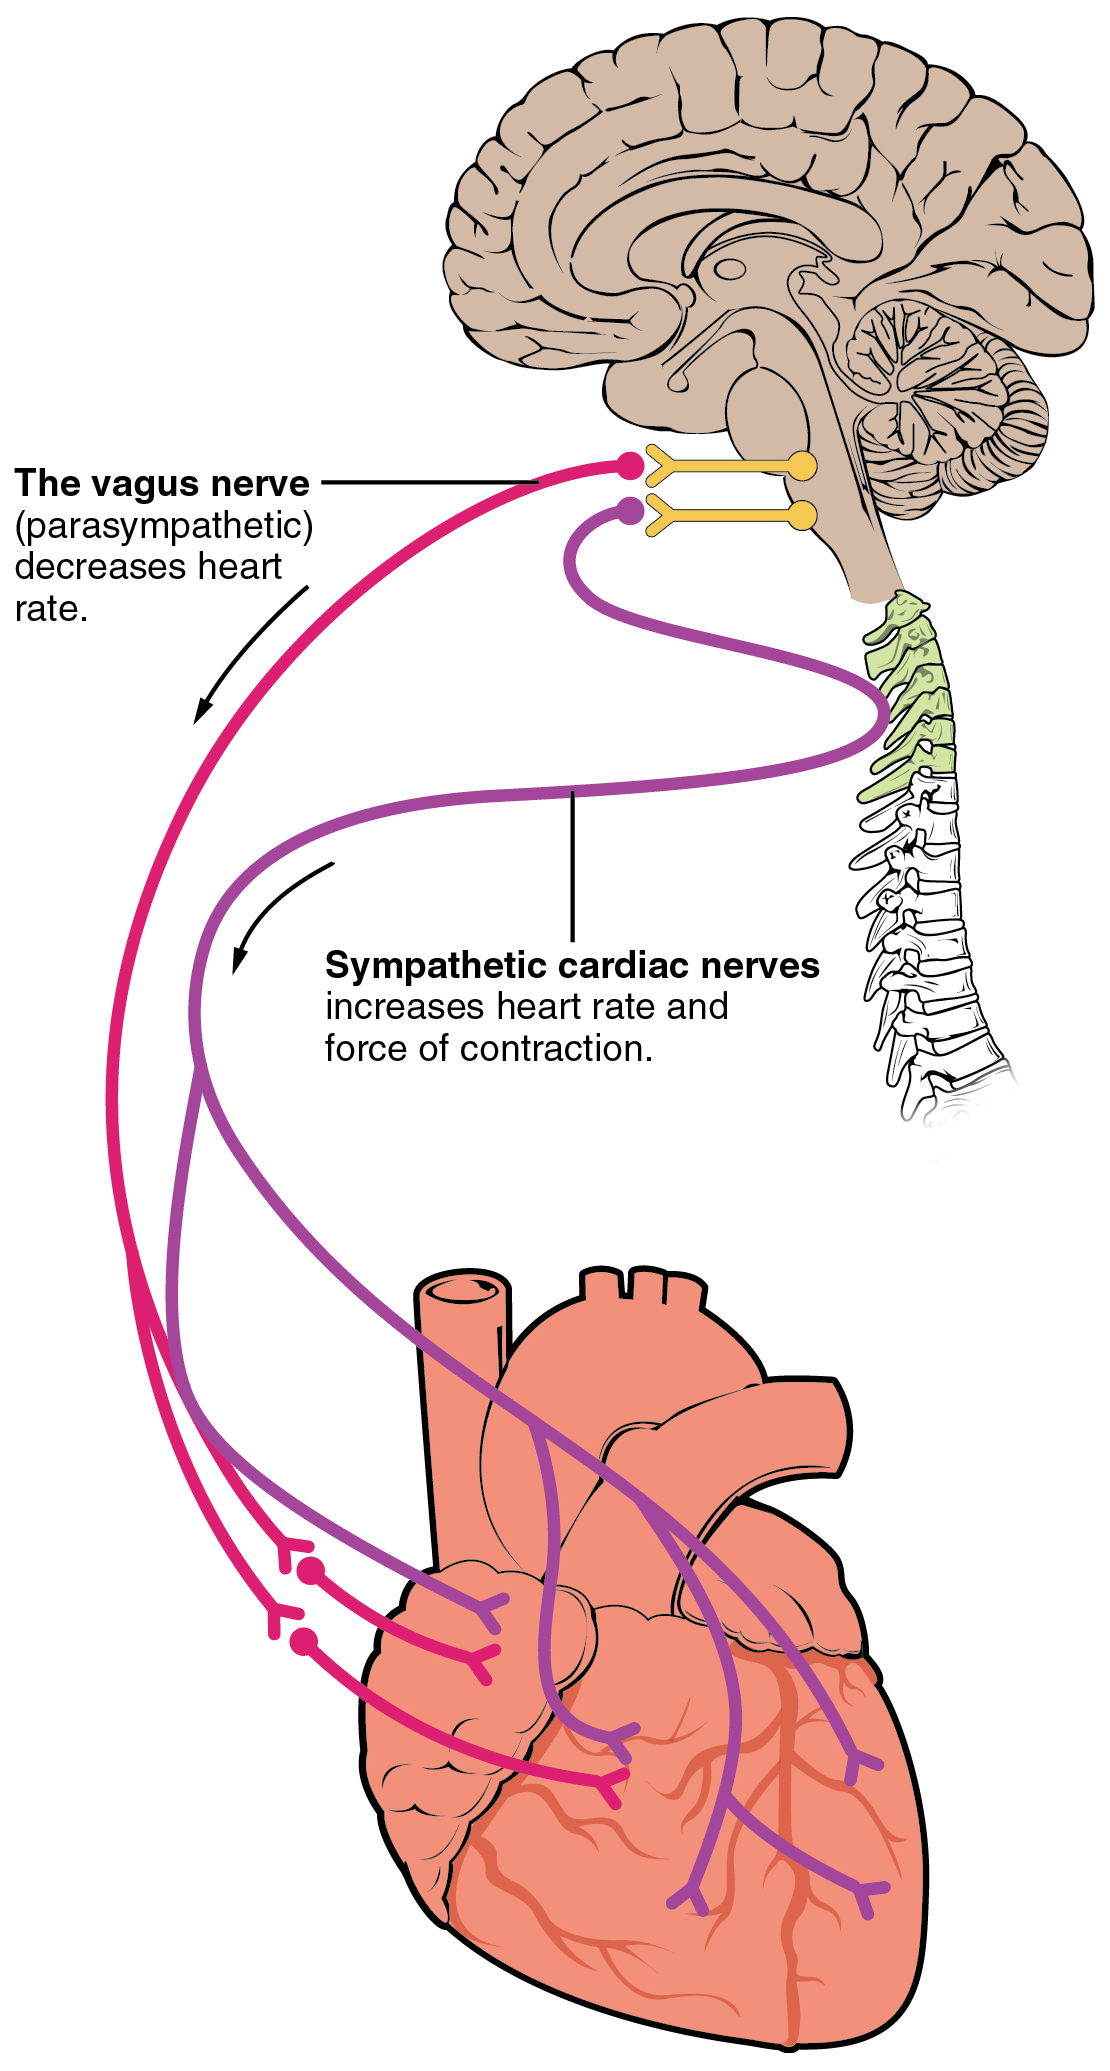
\includegraphics[keepaspectratio]{_resources/images/2032_Automatic_Innervation.jpg}}

}

\caption{迷走神经控制心脏和其他器官。来源:\href{https://commons.wikimedia.org/wiki/File:2032_Automatic_Innervation.jpg}{维基百科}}

\end{figure}%

\section{副交感神经的指挥官:调节功能}\label{ux526fux4ea4ux611fux795eux7ecfux7684ux6307ux6325ux5b98ux8c03ux8282ux529fux80fd}

迷走神经是自主神经系统副交感分支的主要成分------常被描述为''休息与消化''系统。与准备身体在面对压力或危险时采取行动的交感''战斗或逃跑''系统相比,副交感系统促进平静、放松和恢复状态。

通过其传出通路,迷走神经帮助调节众多重要功能:

\textbf{心血管调节}:迷走神经刺激通常会减慢心率并可能降低血压。这种对心脏的''迷走制动''对心脏效率至关重要,允许心脏在运动期间之间休息。对心脏更强的迷走控制与更好的心血管健康和韧性相关。

\textbf{呼吸控制}:迷走神经支配咽喉、喉头和支气管的肌肉,影响呼吸模式和发声活动。它帮助调节呼吸频率并在咳嗽反射中发挥作用,保护气道免受异物侵入。

\textbf{消化协调}:也许最广泛的是迷走神经对消化系统的影响。它刺激胃酸和消化酶的产生,增加肠道蠕动,并控制食物通过消化道的移动。迷走神经对正常消化和营养吸收至关重要。

\textbf{免疫调节}:研究表明,迷走神经在所谓的''炎症反射''中扮演着关键角色。通过这一通路,迷走神经可以检测体内的炎症分子并触发抗炎反应,有助于防止过度炎症。

\textbf{激素释放}:迷走神经影响各种消化激素的释放,包括调节血糖水平的胰岛素。它还影响调节饥饿和饱腹感的胃饥饿素和瘦素的产生。

\section{脑身信息高速公路:传入信号}\label{ux8111ux8eabux4fe1ux606fux9ad8ux901fux516cux8defux4f20ux5165ux4fe1ux53f7}

虽然迷走神经的调节功能令人印象深刻,但同样重要的是它作为从身体到大脑的信息渠道的角色。通过其广泛的感觉纤维网络,迷走神经持续监测内部环境,向大脑提供有关器官功能、能量可用性、潜在威胁和总体生理状态的关键信息。

这种传入(感觉)信息首先到达延髓的孤束核(NTS)。孤束核作为主要整合中心,处理迷走输入并将这些信息传递到各个脑区,包括:

\textbf{蓝斑}:大脑中去甲肾上腺素的主要来源,影响警觉性、注意力和压力反应。

\textbf{下丘脑}:大脑的稳态中心,调节激素、体温、饥饿、口渴和昼夜节律。

\textbf{杏仁核}:对情绪处理很重要,特别是恐惧和焦虑反应。

\textbf{前额叶皮质}:参与执行功能、决策和情绪调节。

通过这些连接,迷走传入信号不仅影响基本生理过程,还影响情绪、认知和应对压力的能力。这解释了为什么我们内脏器官的状态------我们的''肠道感觉''------能深刻影响我们的情绪状态和思维过程。

\begin{figure}[H]

{\centering \pandocbounded{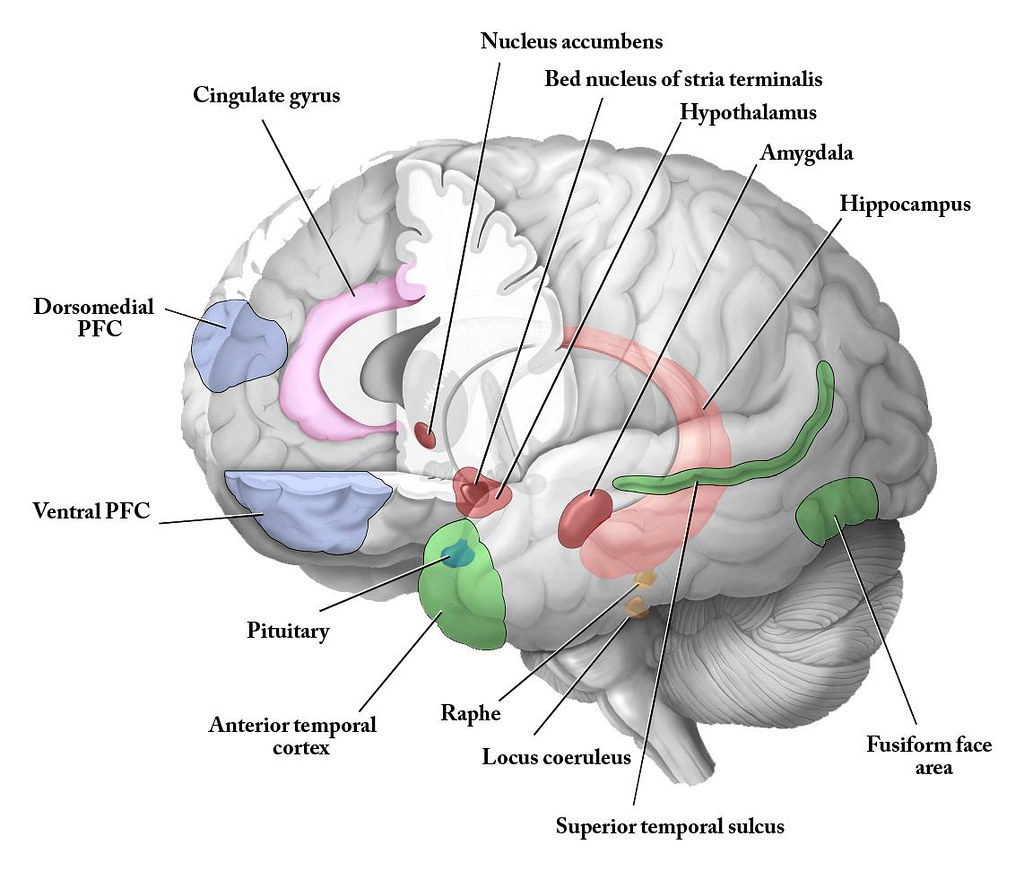
\includegraphics[keepaspectratio]{_resources/images/eian-brain-diagram-210971272_c45fc42276_b.jpg}}

}

\caption{大脑中的传入信号系统。来源:\href{https://www.flickr.com/photos/eian/210971272}{Eian}}

\end{figure}%

\section{迷走张力:神经系统平衡的衡量标准}\label{ux8ff7ux8d70ux5f20ux529bux795eux7ecfux7cfbux7edfux5e73ux8861ux7684ux8861ux91cfux6807ux51c6}

迷走神经对心脏的影响强度,被称为''迷走张力'',已成为自主神经系统功能的重要指标。更高的迷走张力与更大的心率变异性(HRV)相关------连续心跳之间时间的自然变化。健康的心脏不会像节拍器一样规律地跳动,而是显示出反映身体适应变化需求能力的微妙变化。

高迷走张力通常表明一个良好调节的自主神经系统,能够有效地对环境变化做出反应。具有较高迷走张力的个体往往表现出:

\begin{itemize}
\tightlist
\item
  更大的情绪稳定性和应对压力的能力
\item
  从压力事件中更有效的恢复
\item
  更好的注意力和认知表现
\item
  增强的社交能力
\item
  改善的免疫功能
\end{itemize}

相反,低迷走张力与各种健康挑战相关,包括心血管疾病、炎症、焦虑障碍、抑郁症和胃肠问题。迷走功能对健康多方面的中心作用解释了为什么刺激或加强迷走神经的技术在医疗和健康领域受到重视。

\section{多迷走理论:情绪安全的理论}\label{ux591aux8ff7ux8d70ux7406ux8bbaux60c5ux7eeaux5b89ux5168ux7684ux7406ux8bba}

基于我们对迷走神经的理解,Stephen
Porges博士提出了多迷走理论,提供了迷走神经进化意义的细微视角。根据这一理论,迷走神经有两个不同的分支:

\textbf{腹侧迷走复合体}:较新的、有髓鞘的分支,支持社交参与、连接和安全感。当活跃时,它促进有利于积极社交互动、创造力和健康的平静生理状态。

\textbf{背侧迷走复合体}:系统发生学上更古老的、无髓鞘的分支,可能在面临生命威胁的危险时触发静止或''冻结''反应。当占主导地位时,可能导致关闭、解离或抑郁状态。

多迷走理论表明,我们的神经系统在环境中持续评估风险(Porges称之为''神经感知''),根据感知到的安全或威胁在这些不同的迷走状态之间转换。这一理论对理解人类行为、创伤反应和社交动态有着深远的影响。

\section{临床意义:当迷走功能受损}\label{ux4e34ux5e8aux610fux4e49ux5f53ux8ff7ux8d70ux529fux80fdux53d7ux635f}

迷走功能的中断可能表现为各种健康状况。例如,迷走神经病变可能导致如持续咳嗽、声音嘶哑、吞咽困难、心率异常或消化障碍等症状。更微妙地,在许多慢性疾病中观察到迷走影响的减弱,包括:

\begin{itemize}
\tightlist
\item
  炎症性肠病
\item
  糖尿病和代谢紊乱
\item
  焦虑和情绪障碍
\item
  自身免疫性疾病
\item
  慢性疼痛综合征
\end{itemize}

认识到迷走神经在健康中的核心作用,激发了各种旨在优化或恢复迷走功能的干预措施。这些方法从传统做法如深呼吸、冥想和冷水浸泡,到现代医学方法如迷走神经刺激(VNS)疗法,我们将在本书中深入探讨。

\section{结论:迷走神经作为健康晴雨表}\label{ux7ed3ux8bbaux8ff7ux8d70ux795eux7ecfux4f5cux4e3aux5065ux5eb7ux6674ux96e8ux8868}

迷走神经是脑身连接的一个非凡例子,在生理功能的复杂舞蹈中既是调节者又是信息传递者。它广泛的影响------触及几乎每个主要器官系统------使其成为我们整体健康和福祉的关键因素。

随着研究继续揭示迷走神经的众多角色和关系,越来越清楚的是,迷走功能成为了我们生理和心理健康的一种晴雨表。通过理解和支持健康的迷走功能,我们开启了解决广泛健康挑战和优化人类表现的新可能性。

在接下来的章节中,我们将探索现代科学如何通过各种形式的刺激利用迷走神经的力量,为压力管理、认知增强、睡眠改善和情绪调节等提供有前景的方法。

\bookmarksetup{startatroot}

\chapter{神经调节科学:VNS如何影响大脑和身体}\label{ux795eux7ecfux8c03ux8282ux79d1ux5b66vnsux5982ux4f55ux5f71ux54cdux5927ux8111ux548cux8eabux4f53}

\section{理解神经交响乐}\label{ux7406ux89e3ux795eux7ecfux4ea4ux54cdux4e50}

第一章介绍了迷走神经的解剖结构及其在体内的广泛连接,本章将深入探讨使迷走神经刺激(VNS)成为现代健康强大工具的复杂神经生理机制。从本质上讲,VNS代表了技术与我们固有生物调节系统之间的一个非凡接口------一种直接与控制我们生理和心理状态的神经回路''对话''的方式。

迷走神经不仅仅是信号的被动导体;它是一个复杂的双向通信渠道,通过持续的反馈循环连接我们的大脑和身体。正如麻省理工学院McGovern研究所所长、Doris和Don
Berkey脑科学与认知科学教授Robert Desimone博士对神经通信的精辟描述:

``我们的大脑不断被感官信息轰炸。区分相关信息和无关干扰的能力是一项关键技能,这项技能在许多脑部疾病中都会受损。通过研究人类和动物的视觉系统,我们的研究表明,当我们专注于特定事物时,特定脑区的神经元会一致地发放------就像噪音中升起的合唱------使相关信息能被大脑其他区域更有效地'听到'。''

神经同步的这个比喻------``噪音中升起的合唱''------完美地捕捉了迷走神经刺激所提供的:一种更和谐地协调我们神经活动的方法,在大脑和身体中增强信号与噪音的比例。但这种协调在神经生物学水平上究竟如何运作?

\section{神经递质级联}\label{ux795eux7ecfux9012ux8d28ux7ea7ux8054}

当我们刺激迷走神经,无论通过侵入性还是非侵入性手段,我们都会启动一系列神经递质变化,这些变化波及整个中枢神经系统。VNS不是影响单一通路,而是同时调动多个神经调节系统。

\subsection{去甲肾上腺素系统:警觉与投入}\label{ux53bbux7532ux80beux4e0aux817aux7d20ux7cfbux7edfux8b66ux89c9ux4e0eux6295ux5165}

蓝斑(LC)是脑干中的一个小核团,是大脑中去甲肾上腺素(NE)的主要来源,是迷走传入信号首先激活的区域之一。当迷走神经被刺激时,信号传至孤束核(NTS),然后投射到LC,增加其放电频率和整个大脑的NE释放。这种LC-NE激活在促进警觉性、注意力和认知表现方面起着关键作用。

最新研究表明,即使是短暂的经皮VNS会话也能显著增加LC活动,通过瞳孔扩张和EEG模式变化来衡量。一项2021年的研究发现,对睡眠剥夺个体进行6分钟的颈部VNS,能改善他们在复杂认知任务上的表现,效果持续近19小时,可能是通过持续激活LC-NE通路实现的。

\subsection{5-羟色胺调节:平衡情绪}\label{ux7f9fux8272ux80faux8c03ux8282ux5e73ux8861ux60c5ux7eea}

除了去甲肾上腺素系统,VNS还通过NTS与背侧缝核(大脑中5-羟色胺的主要来源)的连接调节5-羟色胺(5-HT)信号。长期VNS已被证明能增加5-羟色胺能神经元的放电频率,并增强前额叶皮质和海马等区域的5-HT传递,与许多抗抑郁药物的效果类似。

这种5-羟色胺调节有助于解释VNS在治疗难治性抑郁和潜在焦虑障碍方面的有效性。与主要针对单一神经递质系统的药物干预不同,VNS似乎在同时影响其他神经调节系统的同时使5-羟色胺功能正常化,可能提供更全面的情绪调节。

\subsection{GABA和谷氨酸:兴奋与抑制的平衡}\label{gabaux548cux8c37ux6c28ux9178ux5174ux594bux4e0eux6291ux5236ux7684ux5e73ux8861}

迷走神经刺激也影响大脑的主要抑制性和兴奋性神经递质:γ-氨基丁酸(GABA)和谷氨酸。研究表明,VNS增加了几个脑区的GABA浓度,包括丘脑、岛叶皮质和边缘区域。

这种GABA增强对于针对焦虑、压力和癫痫的VNS应用特别重要。通过增加抑制性张力,VNS可以帮助抑制过度的神经兴奋,促进平静警觉的状态而非焦虑唤醒。通过VNS实现的兴奋与抑制之间的微妙平衡与许多药理学方法形成对比,后者可能使系统过度偏向抑制(导致镇静)或兴奋(导致激动)。

\section{神经振荡与网络同步}\label{ux795eux7ecfux632fux8361ux4e0eux7f51ux7edcux540cux6b65}

除了个别神经递质系统,VNS深刻影响神经元群体如何通过振荡节律交流和协调它们的活动------大脑的自然计时机制。

\subsection{Alpha和Gamma节律:注意力调节器}\label{alphaux548cgammaux8282ux5f8bux6ce8ux610fux529bux8c03ux8282ux5668}

VNS研究中最一致的发现之一是它对与注意力和认知处理相关的脑节律的影响。具体来说,VNS倾向于减少皮质区域的alpha振荡(8-12
Hz)并增加gamma频带活动(30-100 Hz)。

Alpha波通常在我们放松但不专注于特定任务时占主导地位,形成神经科学家有时称为''怠速节律''的状态。通过减少alpha能量,VNS帮助大脑从这种怠速状态转变为更适合任务的状态。同时,gamma振荡的增强------与主动信息处理和特征绑定相关------支持更高效的认知表现。

使用脑电图(EEG)和脑磁图(MEG)的研究表明,这些振荡活动的变化与VNS后注意力控制、工作记忆和感知辨别能力的改善相关。这些发现完全符合Desimone教授关于注意力任务中神经同步的研究,表明VNS可能增强大脑选择性处理信息的自然机制。

\subsection{前额叶-边缘系统连接:增强情绪调节}\label{ux524dux989dux53f6-ux8fb9ux7f18ux7cfbux7edfux8fdeux63a5ux589eux5f3aux60c5ux7eeaux8c03ux8282}

VNS效应背后的另一个关键神经机制涉及前额叶皮质与边缘结构(如杏仁核、海马和前扣带回皮质)之间连接的调节。功能性神经影像研究揭示,VNS加强了从前额叶区域到参与情绪处理的边缘区域的自上而下控制通路。

这种增强的前额叶-边缘系统连接支持改善情绪调节,允许对压力源和情绪刺激做出更适应性的反应。VNS似乎不是简单地抑制情绪反应,而是促进更灵活和适合上下文的情绪处理------这是与许多用于焦虑和情绪障碍的药物干预的一个关键区别。

\section{免疫-神经接口}\label{ux514dux75ab-ux795eux7ecfux63a5ux53e3}

VNS研究中最引人入胜且快速发展的领域之一是其对免疫系统的影响。迷走神经构成了神经科学家Kevin
Tracey称之为''炎症反射''的关键组成部分------一个检测和调节全身炎症反应的神经回路。

当被VNS激活时,迷走传出纤维在脾脏和其他免疫器官释放乙酰胆碱,与免疫细胞上的α7烟碱型乙酰胆碱受体结合。这种胆碱能信号抑制促炎症细胞因子如肿瘤坏死因子(TNF)、白细胞介素-1β(IL-1β)和白细胞介素-6(IL-6)的产生,同时促进抗炎症介质。

这种免疫调节的临床意义深远。VNS在治疗从类风湿性关节炎到炎症性肠病的炎症状况方面显示出希望,不是通过广泛抑制免疫功能(如许多免疫抑制药物那样),而是通过将免疫反应重新校准为稳态。

此外,这种抗炎作用创造了一个有利于脑功能的正反馈循环。通过减少外周炎症,VNS有助于保护大脑免受与炎症细胞因子升高相关的认知和情绪损伤------研究人员有时称之为''疾病行为''。这可能部分解释了常规使用VNS观察到的认知和情绪益处。

\section{自主神经平衡行为}\label{ux81eaux4e3bux795eux7ecfux5e73ux8861ux884cux4e3a}

如第1章所讨论的,迷走神经是大多数内脏器官的主要副交感输出。然而,VNS并不是简单地全面增加副交感活动;相反,它帮助将整个自主神经系统重新校准为更适应性的功能。

\subsection{心率变异性:自主平衡的窗口}\label{ux5fc3ux7387ux53d8ux5f02ux6027ux81eaux4e3bux5e73ux8861ux7684ux7a97ux53e3}

这种自主重新平衡最可靠的生物标记之一是心率变异性(HRV)------心律中自然的心跳间变化,反映了交感神经和副交感神经之间的动态相互作用。健康的HRV特征是复杂的变化模式,而不是刚性规律性或混乱波动。

VNS通常会增加HRV,特别是与呼吸窦性心律不齐相关的高频带(HF-HRV)------由迷走神经介导的呼吸与心率之间的自然同步。除了简单地增加副交感张力外,这种增强的HRV代表了一个更为反应灵敏和适应性的自主神经系统,能够精确地将生理资源与不断变化的需求匹配。

\subsection{多迷走视角:安全信号与社交参与}\label{ux591aux8ff7ux8d70ux89c6ux89d2ux5b89ux5168ux4fe1ux53f7ux4e0eux793eux4ea4ux53c2ux4e0e}

Stephen
Porges的多迷走理论为理解VNS效应提供了另一个有见地的框架。根据这一理论,迷走神经(特别是其髓鞘化分支)在社交参与和安全感中起着至关重要的作用。

通过刺激这些迷走通路,VNS可能帮助自主神经系统从防御状态(以交感唤醒或非髓鞘化迷走撤回为特征)转向支持社交连接、平静警觉和心理安全的状态。这一视角有助于解释为何VNS能同时减轻焦虑同时改善认知和社交功能------这些效果在传统自主模型中可能看似矛盾。

\section{超越单一机制:系统观点}\label{ux8d85ux8d8aux5355ux4e00ux673aux5236ux7cfbux7edfux89c2ux70b9}

使VNS作为神经调节方法特别强大的是,它不只针对这些机制中的一个------它同时调动所有这些机制,创造协同效应,可以通过仔细的参数调整根据个人需求定制。

例如,不同的刺激频率似乎会优先激活不同的机制:较低频率(1-10
Hz)可能强调自主平衡和抗炎效应,而较高频率(20-30
Hz)可能通过去甲肾上腺素和注意力通路最大化认知增强。

这种系统级影响将VNS与大多数药物方法区分开来,后者通常针对单一受体类型或神经递质系统。结果是一种更生理连贯的干预,与身体的自然调节机制协同工作,而不是覆盖它们。

在下一章中,我们将探讨这种对VNS机制的丰富理解如何指导该技术从其作为癫痫治疗的起源到其在日常生活中优化健康和表现的新兴角色的演变。

\bookmarksetup{startatroot}

\chapter{从医疗干预到健康工具:VNS技术的演变}\label{ux4eceux533bux7597ux5e72ux9884ux5230ux5065ux5eb7ux5de5ux5177vnsux6280ux672fux7684ux6f14ux53d8}

迷走神经刺激(VNS)从需要手术植入的临床程序到可访问的消费级健康技术的发展历程,代表了现代神经技术领域最引人入胜的轨迹之一。这一演变反映了医疗保健更广泛的转变:从纯粹以治疗为导向的方法向预防性和增强型干预转变,以及从集中化医疗技术向民主化个人健康工具转变。本章追溯这一非凡的转变,同时探讨塑造当前VNS设备格局的关键里程碑、科学突破和市场力量。

\section{临床VNS的诞生:开创性医疗应用}\label{ux4e34ux5e8avnsux7684ux8bdeux751fux5f00ux521bux6027ux533bux7597ux5e94ux7528}

现代临床VNS应用始于20世纪80年代,源于数十年关于迷走神经在调节身体功能中作用的研究。早期动物研究表明,迷走神经的电刺激可以影响癫痫发作活动,为人类应用奠定了基础。1988年,第一次针对癫痫治疗的人类VNS设备植入标志着一个分水岭时刻------将关于神经调节的理论知识转化为实际医疗干预。

早期的VNS系统完全是侵入性的,需要在胸壁植入脉冲发生器(类似于起搏器),电极通过皮下隧道连接并缠绕在颈部左侧迷走神经上。这些系统根据医生预设的参数向神经传递精确校准的电脉冲。这种方法允许持续的长期刺激,但有显著的局限性:手术风险、高成本(设备和手术通常超过20,000美元)以及植入物的永久性。

尽管有这些缺点,临床结果足够有希望,1997年FDA批准VNS治疗12岁及以上的难治性癫痫患者。这一首次批准专门针对减少对多种抗癫痫药物反应不足的患者的发作频率。该疗法不是作为一线治疗定位,而是作为选择有限的患者的最后手段。

第二个主要临床应用出现在2005年,当时FDA批准VNS用于难治性抑郁症(TRD)。这一批准是在观察到接受VNS的癫痫患者情绪常常改善,而这种改善独立于发作控制之外。对抑郁症的批准意义重大,因为它承认了VNS在纯神经系统疾病之外的更广泛神经精神潜力。

这些早期医疗应用建立了重要的先例:它们证明了VNS的安全性,确认了其通过外周神经调节脑功能的能力,并建立了参数选择的方案。然而,它们仍然牢固地处于医疗领域------昂贵、侵入性,且只有那些患有严重医疗条件的人在医生监督下才能获得。

\section{过渡阶段:非侵入性临床应用}\label{ux8fc7ux6e21ux9636ux6bb5ux975eux4fb5ux5165ux6027ux4e34ux5e8aux5e94ux7528}

向更广泛应用的第一个重大转变来自于2010年代非侵入性VNS方法的发展。这些方法旨在通过皮肤刺激迷走神经,消除了手术需求,同时保留治疗效果。两种主要方法出现:

\begin{enumerate}
\def\labelenumi{\arabic{enumi}.}
\tightlist
\item
  \textbf{经皮耳廓迷走神经刺激(taVNS)}:通过小型电极靶向外耳的迷走神经耳支
\item
  \textbf{经皮颈部迷走神经刺激(tcVNS)}:通过手持设备通过颈部皮肤刺激主迷走神经干
\end{enumerate}

electroCore公司开发的gammaCore设备代表了这一过渡。最初为偏头痛和丛集性头痛治疗而设计,该手持设备于2017年获得FDA批准。用户在头痛发作期间将设备应用于颈部进行短时刺激(通常为2分钟)。虽然仍被归类为需要处方的医疗设备,但gammaCore代表了向患者自主治疗的重要一步。

耳基刺激设备也出现了类似的发展。像Parasym这样的公司开发了针对迷走神经耳支的设备,用于从炎症性疾病到焦虑等多种疾病。虽然这些设备保持了医疗设备的分类,但它们的非侵入性大大降低了获取障碍。

在此期间,对VNS机制的科学理解也扩展了。正如第2章所讨论的,研究人员确定了VNS影响脑活动、炎症和自主功能的特定神经通路。这种更深入的理解使得更有针对性的应用成为可能,并帮助区分了早期方案中的基本刺激参数与不必要的方面。

这一过渡阶段的特点是: - 医生监督但患者控制增加 -
较低风险状况使适应症扩大 - 间歇性刺激方案而非持续刺激 -
显著降低成本(从20,000+美元降至500-2,000美元) -
对VNS在压力、炎症和认知功能方面效果的证据日益增多

现在的舞台已经为下一次进化飞跃------从处方医疗治疗到消费健康工具------做好了准备。

\section{健康革命:消费级VNS技术}\label{ux5065ux5eb7ux9769ux547dux6d88ux8d39ux7ea7vnsux6280ux672f}

在2018-2022年左右,出现了一批明确针对健康市场的新一代VNS设备。这些面向消费者的技术利用了医学VNS研究建立的科学基础,但重新定义了技术的目的:从治疗特定疾病到优化正常功能和增强韧性。

这一转变由几个汇聚因素促成:

\begin{enumerate}
\def\labelenumi{\arabic{enumi}.}
\tightlist
\item
  \textbf{制造进步}大幅降低了生产成本
\item
  \textbf{电子元件微型化}允许优雅、可穿戴的设计
\item
  \textbf{移动技术集成}实现应用控制和数据跟踪
\item
  \textbf{消费者对神经技术和个性化健康的兴趣增长}
\item
  \textbf{健康设备的监管途径}不需要与医疗设备相同的严格审批流程
\end{enumerate}

早期消费设备如Neuvana的Xen(2019年发布)代表了这种新方法。外形类似标准耳机,Xen在用户听音乐的同时向迷走神经耳支传递温和的电刺激。配套的智能手机应用程序允许用户调整刺激强度并跟踪使用情况。重要的是,它不是针对特定医疗条件,而是针对压力减轻、注意力增强和睡眠改善------这些影响几乎每个人的健康问题。

这些设备周围的营销语言发生了巨大变化,从医学术语转向生活方式益处。临床VNS曾以''治疗''、``疗法''和''症状''来描述,而消费级VNS则强调''优化''、``表现''、``韧性''和''平衡''。这种转变不仅反映了营销策略,更反映了对技术目的的根本重新概念化。

其他公司很快进入市场,提供各种形式因素:头带式设备、耳夹、颈部佩戴刺激器,甚至隐藏技术功能的珠宝灵感设计。价格点通常在200-700美元范围内------仍属重要投资,但仅为医疗VNS成本的一小部分,定位在高端消费电子范围内,而非医疗设备类别。

\section{消费时代的科学验证}\label{ux6d88ux8d39ux65f6ux4ee3ux7684ux79d1ux5b66ux9a8cux8bc1}

关于消费级VNS设备的一个关键问题是它们的有效性:这些简化、低强度的设备是否能产生有意义的生理效果?针对消费设备的研究相比临床VNS的广泛文献仍然有限,但几条证据支持它们的潜在有效性:

\begin{enumerate}
\def\labelenumi{\arabic{enumi}.}
\item
  \textbf{参数重叠}:许多消费设备在研究环境中显示能激活迷走通路的刺激参数范围(频率、脉宽、幅度)内运行。
\item
  \textbf{生物标记研究}:独立研究已表明,即使是简短、温和的经皮VNS也能影响已确立的生物标记,包括心率变异性、瞳孔反应和皮质醇水平。
\item
  \textbf{用户体验数据}:公司已经积累了大量用户报告的结果数据,表明对压力、睡眠和主观幸福感有益效应,尽管这些证据有固有的局限性。
\item
  \textbf{有针对性的学术合作}:几个设备制造商已与学术机构合作验证特定产品声明,初步结果支持某些效果。
\end{enumerate}

然而,消费领域缺乏医疗设备所需的严格临床试验,造成了证据差距。鉴于医疗和健康产品之间的监管差异,这一差距并不令人惊讶,但它代表着未来研究的机会。最负责任的消费公司承认这些局限性,同时继续建立证据基础。

\section{当前格局与未来轨迹}\label{ux5f53ux524dux683cux5c40ux4e0eux672aux6765ux8f68ux8ff9}

如今的VNS格局跨越了从可植入医疗设备到时尚消费可穿戴设备的连续谱系。在医疗领域,新一代可植入系统提供改进的可编程性和电池寿命,而非侵入性处方设备继续扩展其批准适应症。健康领域已根据专门用例多样化:为睡眠开始、压力管理、专注力增强,甚至运动恢复优化的设备。

始于高度专业医疗干预的技术已转变为在健康与健康领域应用广泛的多功能技术平台。这种演变继续加速,几个有前景的前沿正在出现:

\begin{enumerate}
\def\labelenumi{\arabic{enumi}.}
\item
  \textbf{闭环系统}基于实时生理测量调整刺激(将在第10章进一步探讨)
\item
  \textbf{组合方法}将VNS与呼吸训练、声音疗法或认知练习等互补模式整合在一起
\item
  \textbf{形式因素创新}使设备越来越不显眼,与生活方式兼容
\item
  \textbf{个性化算法}基于个体反应模式优化刺激参数
\item
  \textbf{扩展生物靶点}超越传统VNS效应,可能包括肠-脑轴调节和免疫功能
\end{enumerate}

这种演变------从手术室到客厅,从最后手段治疗到日常健康实践------展示了健康技术更广泛的模式。随着我们对身体调节系统的理解深入,最初为治疗功能障碍而开发的技术越来越多地应用于优化正常功能。VNS代表了这一轨迹的典型例子,已经完成了从高度专业医疗干预到可访问的日常健康工具的旅程。

接下来的章节将探讨现代VNS技术在压力管理、认知表现和睡眠中的具体应用------在此基础上研究这些进化系统如何增强现代生活的各个方面。

\bookmarksetup{startatroot}

\chapter{管理压力和焦虑:VNS作为神经调节干预}\label{ux7ba1ux7406ux538bux529bux548cux7126ux8651vnsux4f5cux4e3aux795eux7ecfux8c03ux8282ux5e72ux9884}

在我们日益苛求的现代世界中,慢性压力和焦虑的生理代价已成为一个紧迫的公共卫生问题。正如我们在第2章中探讨的,迷走神经作为大脑和身体之间的关键通信高速公路,在我们的压力反应系统中扮演着核心角色。本章将更深入地探讨迷走神经刺激(VNS)如何特别影响压力生理学和焦虑状态,审视支持其作为这些状况神经调节干预的日益增长的证据。

\section{压力的神经生理学与迷走连接}\label{ux538bux529bux7684ux795eux7ecfux751fux7406ux5b66ux4e0eux8ff7ux8d70ux8fdeux63a5}

人类压力反应涉及复杂的神经和激素事件级联,传统上分为''战斗或逃跑''(交感激活)和''休息与消化''(副交感恢复)。虽然第2章概述了迷走功能的一般机制,但这里我们特别关注迷走活动如何通过三个关键途径调节压力。

\subsection{HPA轴调节回路}\label{hpaux8f74ux8c03ux8282ux56deux8def}

下丘脑-垂体-肾上腺(HPA)轴代表我们身体的中枢压力反应系统。当大脑感知到威胁时,下丘脑释放促肾上腺皮质激素释放激素(CRH),触发一系列级联反应,最终导致肾上腺产生皮质醇。这种压力激素动员能量资源,但长期升高会导致许多健康问题。

最近的研究揭示了迷走张力与HPA轴功能之间令人着迷的调节关系。在一项具有开创性的2023年研究中,Butt及同事证明,经皮耳迷走神经刺激(taVNS)显著抑制了心理压力任务期间的皮质醇释放。接受仅30分钟10
Hz
taVNS的参与者,与接受假刺激的对照组相比,在标准化压力方案期间唾液皮质醇水平明显较低。最引人注目的是,taVNS组的峰值皮质醇反应约减少了25\%,表明压力反应显著降低。

这一发现建立在早期动物研究的基础上,这些研究表明迷走传入信号通过孤束核(NTS)传递,对下丘脑室旁核产生抑制作用------本质上对HPA轴施加神经''制动''。通过刺激增强这一迷走抑制回路,VNS似乎在其源头调节压力反应。

\subsection{炎症调节途径}\label{ux708eux75c7ux8c03ux8282ux9014ux5f84}

除了HPA轴效应外,VNS还强有力地影响身体对压力的炎症反应------这一机制与前几章所涵盖的不同。所谓的''炎症反射''涉及通过迷走传出信号抑制促炎细胞因子的产生。在压力状态下,炎症往往会增加,与心理困扰形成有害的反馈循环。

新证据表明taVNS可以打断这一循环。2024年的一项随机对照试验检查了42名广泛性焦虑障碍成人在每日taVNS治疗八周前后的炎症标志物。与假刺激相比,taVNS组的促炎细胞因子,包括IL-6(减少31\%)和TNF-α(减少26\%)显著降低,与焦虑症状改善密切相关。重要的是,抗炎效应似乎部分独立于HPA轴调节,因为一些参与者显示炎症标志物正常化,尽管皮质醇模式变化很小。

这种胆碱能抗炎通路代表VNS减轻慢性焦虑心理生理负担的一种独特机制------鉴于对炎症在情绪障碍中作用的新兴理解,这一点尤为相关。

\subsection{自主平衡与心率变异性}\label{ux81eaux4e3bux5e73ux8861ux4e0eux5fc3ux7387ux53d8ux5f02ux6027}

VNS对压力生理学最直接的影响可能发生在通过直接调节自主平衡的过程中,这反映在心率变异性(HRV)测量中。随着焦虑增加,交感活动通常占主导地位,降低HRV并创造一种生理状态,为持续压力做好准备。

先进的HRV分析现在提供了一个窗口,展示VNS以微妙的方式重新平衡压力期间的自主功能。Tarvainen及同事(2022)使用机器学习算法分析对taVNS的HRV模式反应,发现刺激不仅增加了反映迷走活动的高频(HF)成分,还诱导了自主调节的更复杂重组。他们的工作揭示了对特定频率波段的不成比例影响,一些个体在压力挑战期间甚至显示LF/HF比率降至基线水平以下------本质上是''比正常更好''的副交感反应。

这种自主重新校准发生得很快,通常在刺激开始后几分钟内,使其特别适合急性压力管理情况。这些发现也有助于解释为什么主观焦虑缓解往往先于其他生物标志物的可测量变化------自主平衡的微妙变化可能立即被感觉为平静感,尽管其他系统的变化滞后。

\section{焦虑障碍的临床应用}\label{ux7126ux8651ux969cux788dux7684ux4e34ux5e8aux5e94ux7528}

从生理机制转向临床应用,研究越来越支持VNS在整个焦虑谱系障碍中的有效性。与往往孤立处理症状的常规治疗不同,VNS通过调节焦虑状态的核心神经回路,提供了独特的''上游''方法。

\subsection{特定焦虑状况的证据}\label{ux7279ux5b9aux7126ux8651ux72b6ux51b5ux7684ux8bc1ux636e}

\subsubsection{创伤后应激障碍(PTSD)}\label{ux521bux4f24ux540eux5e94ux6fc0ux969cux788dptsd}

PTSD代表一种特别具有挑战性的焦虑状况,特征是自主失调和病理性恐惧反应。最近的双盲试验表明,经皮颈部VNS可以显著减少对创伤相关线索的生理反应性。一项值得注意的研究发现,与假刺激相比,当PTSD患者暴露于创伤提醒物时,主动刺激将心率加速减少了45\%,并增加了外周血容量波幅(表明血管收缩减少)。

快速的生理稳定表明VNS可能在神经水平上充当''安全信号'',反向条件化维持创伤症状的夸大自主反应。有趣的是,这种益处持续超过刺激期,20分钟刺激后记录到惊吓反应减少长达两小时。

\subsubsection{广泛性焦虑障碍(GAD)}\label{ux5e7fux6cdbux6027ux7126ux8651ux969cux788dgad}

对于GAD患者,其特征是持续的担忧和紧张,初步试验已经出现了令人鼓舞的证据。2022年的一项耳部taVNS在初级保健中的开放标签研究显示,焦虑有意义的减少,GAD-7评分从平均14.8分(中度至重度焦虑)在四周每日两次刺激后降至8.3分(轻度焦虑)。虽然承认开放标签设计的局限性,但改善的幅度超过了焦虑治疗研究中观察到的典型安慰剂效应。

更具说服力的是,2023年使用功能性神经影像的试点研究发现,taVNS使GAD患者杏仁核与前额叶皮质之间通常见到的超连接正常化。这种健康神经回路功能的恢复与主观焦虑改善相关,表明VNS可能解决慢性担忧状态的基本网络失调。

\subsubsection{惊恐障碍}\label{ux60caux6050ux969cux788d}

焦虑的最戏剧性自主表现可能发生在惊恐发作期间,特征是突然、强烈的生理唤醒。早期病例系列和小型试验表明非侵入性VNS可能对惊恐预防特别有益。一项单盲交叉研究发现,与假刺激相比,惊恐障碍患者在为期三周的活性taVNS期间,意外惊恐发作减少了32\%。

对急性惊恐状态的快速有效性可能源于VNS能够快速中断在发作期间放大身体症状的自主级联反应。许多患者报告在惊恐的第一个征兆时使用按需刺激,有效防止全面发作------这比传统治疗只能预防性工作或在症状升级后才起作用有了显著进步。

\section{在压力管理计划中的实际实施}\label{ux5728ux538bux529bux7ba1ux7406ux8ba1ux5212ux4e2dux7684ux5b9eux9645ux5b9eux65bd}

从临床障碍转向日常压力管理,VNS为将神经调节干预整合到综合健康计划中提供了新的可能性。与许多需要大量时间投入或环境修改的减压技术不同,VNS可以在各种环境中谨慎应用,对日常活动的干扰最小。

\subsection{工作场所应用}\label{ux5de5ux4f5cux573aux6240ux5e94ux7528}

几个创新的组织健康计划已开始纳入非侵入性VNS设备,特别是在高压职业中。2024年针对急诊科医生的一项试点计划发现,提供在班次期间使用的耳刺激设备与三个月后改善的压力恢复指标和减少倦怠指标相关。医生报告赞赏能够在患者之间使用简短的刺激会话,大多数人发现2-5分钟足以在繁忙的轮班期间恢复注意力和平静。

同样,企业健康倡议已经探索了午休VNS方案,发现中午刺激可能有助于抵消在高需求工作日期间通常出现的皮质醇和炎症峰值。这些应用代表了临床干预与日常环境中实际压力管理之间的有前途的桥梁。

\subsection{与传统减压方法配对}\label{ux4e0eux4f20ux7edfux51cfux538bux65b9ux6cd5ux914dux5bf9}

VNS不是替代已建立的技术,而是似乎增强了传统压力管理方法的有效性。最近的研究已经检验了将VNS与正念冥想、深呼吸练习和认知行为策略结合的协同效应。一项引人入胜的研究发现,与任一单独干预相比,同时进行taVNS的参与者在生理压力标志物和主观焦虑评级方面都有更大改善。

这种增强效应可能源于VNS为心理干预创造了更具接受性的神经生理状态------本质上''预先调节''神经系统以便放松和认知灵活性。对于实际应用,这表明在进行其他压力管理技术之前立即进行简短VNS会话可能有潜在益处。

\section{结论:希望与局限}\label{ux7ed3ux8bbaux5e0cux671bux4e0eux5c40ux9650}

迷走神经刺激代表了我们对压力和焦虑神经学方法的重大进步,提供了直接调节这些状况基本生物通路的方式。来自HPA轴效应、炎症调节和自主重新平衡的汇聚证据表明,VNS在多个水平上作用于压力反应系统,可能不仅解决症状,还解决痛苦的根本生理驱动因素。

然而,关于最佳刺激参数、个体反应差异和长期效应的重要问题仍然存在。正如我们将在第8章中探讨的,基于个体压力生理学特征的刺激方案个性化可能最大化益处。同样,刺激的适当时机------是预防性的、在急性压力期间或是为了恢复------通过正在进行的研究继续得到完善。

随着VNS技术变得更加可及,我们对其效应的理解不断增长,我们站在压力管理新方法的门槛上------一种认识并直接解决在我们对生活挑战的反应中连接大脑和身体的神经回路的方法。在下一章中,我们将研究这些相同的神经原理如何延伸到认知表现,探索VNS如何增强注意力、专注和心理清晰度。

\bookmarksetup{startatroot}

\chapter{认知优势:VNS用于专注力、注意力和心理表现}\label{ux8ba4ux77e5ux4f18ux52bfvnsux7528ux4e8eux4e13ux6ce8ux529bux6ce8ux610fux529bux548cux5fc3ux7406ux8868ux73b0}

在我们日益复杂、信息饱和的世界中,集中注意力和保持最佳认知表现的能力已成为一项关键技能------一项许多人发现越来越难以掌握的技能。虽然前几章已探讨了迷走神经刺激(VNS)如何调节自主神经系统以减轻压力和焦虑,但本章研究一个不同但同样有价值的方面:VNS如何增强认知功能并提供所谓的''认知优势''。

\section{注意力危机与解决方案的寻找}\label{ux6ce8ux610fux529bux5371ux673aux4e0eux89e3ux51b3ux65b9ux6848ux7684ux5bfbux627e}

现代生活给我们的注意力系统带来了前所未有的挑战。数字干扰、信息过载和持续连接创造了一种被一些神经科学家称为''注意力经济''的环境------在这里,我们的注意力成为最珍贵和最耗尽的资源之一。在这种环境中,大脑选择性注意的自然能力不断受到考验。

正如麻省理工学院麦戈文脑研究所所长Robert Desimone博士所雄辩地解释的:

\begin{quote}
``我们的大脑不断被感官信息轰炸。区分相关信息和无关干扰的能力是一项关键技能,而这项技能在许多脑部疾病中都会受损。通过研究人类和动物的视觉系统,我们的研究表明,当我们专注于特定事物时,特定脑区的神经元会一致地发放------就像噪音中升起的合唱------使相关信息能被大脑其他区域更有效地'听到'。''
\end{quote}

神经同步的这个比喻------``噪音中升起的合唱''------准确地捕捉了我们今天在认知工具箱中所需要的。而令人惊奇的是,VNS提供了一个潜在的途径来增强这种自然注意力机制。

\section{VNS注意力增强的神经机制}\label{vnsux6ce8ux610fux529bux589eux5f3aux7684ux795eux7ecfux673aux5236}

如第2章所讨论的,迷走神经作为连接大脑和身体的主要导管,拥有广泛的传入(感觉)纤维向大脑传递信息。当涉及注意力和认知表现时,关键通路涉及脑干中的孤束核(NTS),它接收这些迷走输入,然后投射到几个重要区域,包括蓝斑(LC)。

蓝斑是大脑去甲肾上腺素(NE)的主要来源,这种神经递质在唤醒、注意力和认知表现中起着关键作用。使VNS对认知增强特别有趣的是它调节LC-NE系统的能力。

当VNS激活NTS时,它可以增加LC神经元的放电率,导致整个皮质区域NE释放增加。这种NE释放对注意力网络有几个有益效应:

\begin{enumerate}
\def\labelenumi{\arabic{enumi}.}
\item
  \textbf{增强信噪比}:NE帮助抑制无关神经活动,同时增强对相关刺激的反应------本质上改善大脑的过滤能力。
\item
  \textbf{增加神经可塑性}:LC-NE系统促进支持学习和记忆形成的突触变化。
\item
  \textbf{认知灵活性}:最佳NE水平支持在不同任务和心理状态之间切换的能力------执行功能的一个关键组成部分。
\item
  \textbf{警觉性维持}:LC-NE系统帮助维持长时间的警觉性,防止自然地向不注意漂移。
\end{enumerate}

Sharon及同事(2021)的一项开创性研究表明,人类经皮VNS诱导可测量的瞳孔扩张------LC-NE系统激活的一个公认生物标记------并减弱与空闲或休息状态相关的alpha振荡。这些生理变化与增强的注意力处理和认知任务准备相关。

\section{认知增强的证据}\label{ux8ba4ux77e5ux589eux5f3aux7684ux8bc1ux636e}

上述理论机制得到了越来越多实证证据的支持,这些证据表明VNS对各种认知领域的影响:

\subsection{持续注意力和警觉性}\label{ux6301ux7eedux6ce8ux610fux529bux548cux8b66ux89c9ux6027}

一项研究VNS和认知表现最令人信服的研究是与睡眠剥夺个体一起进行的。Capone及同事(2021)对连续清醒24小时的参与者进行了经皮颈部迷走神经刺激(使用gammaCore设备,25
Hz)。与假刺激对照组相比,VNS组在持续注意力任务和多任务测试中表现显著更好。

值得注意的是,这些认知改善在单次刺激后持续了近19小时。研究人员得出结论,VNS可能激活了LC-NE通路,帮助维持大脑的警觉性和认知功能,尽管存在睡眠剥夺。

这一发现对必须在延长工作时间、跨时区旅行或其他需要在生理挑战下保持最佳警觉性的情况下维持注意力和认知表现的专业人士有重要意义。

\subsection{工作记忆和信息处理}\label{ux5de5ux4f5cux8bb0ux5fc6ux548cux4fe1ux606fux5904ux7406}

VNS似乎不仅增强注意力,还增强工作记忆------负责暂时保持和操作信息的认知系统。在植入VNS设备治疗癫痫的患者中,研究表明,与禁用期相比,刺激活跃期间工作记忆表现明显改善。

Sun及同事(2017)观察到,当VNS启用时,癫痫患者在依赖记忆的任务上的错误率显著降低,同时脑活动中与早期感觉注意相关的成分增强(特别是,N1波幅增加)。这些发现表明,VNS可以提升信息处理的早期阶段和随后在工作记忆中对该信息的操作。

对于必须在执行复杂认知操作的同时保持多条信息的知识工作者来说------从平衡市场变量的金融分析师到追踪复杂代码结构的软件开发人员------这些工作记忆增强可能转化为有意义的生产力提升。

\subsection{学习和认知可塑性}\label{ux5b66ux4e60ux548cux8ba4ux77e5ux53efux5851ux6027}

也许最引人入胜的是VNS通过增强神经可塑性------大脑形成新连接的能力------来加速学习的潜力。纽约大学兰贡医学中心的最近研究表明,与行为训练配对的VNS显著提高了动物模型中的学习率。当小鼠在训练区分类似音调时接受VNS,它们在对照组达到平台期后仍继续进步,最终实现错误率仅为非刺激动物的一半。

这种增强学习背后的机制涉及VNS激活大脑的胆碱能系统------使用乙酰胆碱作为主要神经递质的神经元网络,在注意力和记忆形成中发挥关键作用。当研究人员阻断动物的胆碱能神经元时,VNS的学习增强效果消失,确认了这一系统在VNS促进学习中的重要作用。

使这一发现对人类认知增强特别相关的是,胆碱能系统已知对我们形成新记忆和学习新技能的能力至关重要。如果VNS确实能''超充''这一系统,它可能有助于人们更快地学习并更有效地保留信息------无论是为考试学习,掌握新的专业技能,还是脑损伤后的康复。

\section{个体差异和状态依赖效应}\label{ux4e2aux4f53ux5deeux5f02ux548cux72b6ux6001ux4f9dux8d56ux6548ux5e94}

VNS认知效应的一个重要细微差别是它们似乎是状态依赖的,并因个体而异。研究表明,VNS在以下情况下提供最显著的认知益处:

\begin{enumerate}
\def\labelenumi{\arabic{enumi}.}
\item
  \textbf{基线表现次优}:疲劳、压力或其他原因导致认知表现低于潜力的个体往往比已处于最佳表现状态的个体在使用VNS时表现出更明显的改善。
\item
  \textbf{任务需要持续注意力}:VNS效应在需要警觉性或延长集中的任务中特别明显,相比简单或自动的认知过程。
\item
  \textbf{个体迷走张力各异}:基线迷走张力较低(通常通过心率变异性测量)的人可能从VNS获得更显著的认知增强。
\end{enumerate}

这种状态依赖性表明,VNS可能不太像传统意义上的''认知增强剂'',更像是''认知优化器''或''正常化器''------帮助恢复因压力、疲劳或心理困扰而受损的最佳认知功能。

\section{认知增强的实际应用}\label{ux8ba4ux77e5ux589eux5f3aux7684ux5b9eux9645ux5e94ux7528}

基于第9章中概述的使用场景,VNS认知增强的几个特定应用值得考虑:

\subsection{早晨认知启动}\label{ux65e9ux6668ux8ba4ux77e5ux542fux52a8}

早晨进食后但开始工作前,进行短时间(5-10分钟)约25
Hz的经皮VNS,可以帮助激活LC-NE通路,为专注的认知工作准备大脑。这种方法利用VNS增强神经处理中信噪比的能力,可能创造一个增强注意力和处理能力的窗口。

\subsection{任务切换促进}\label{ux4efbux52a1ux5207ux6362ux4fc3ux8fdb}

对于必须频繁在不同认知任务之间切换的专业人士------这个过程通常会在注意力和表现方面产生''切换成本''------在主要任务转换之间进行简短的VNS会话(2-3分钟)可能有助于调动与最佳NE水平相关的认知灵活性机制。这可能减少改变情境时通常出现的表现下降。

\subsection{学习增强协议}\label{ux5b66ux4e60ux589eux5f3aux534fux8bae}

在获取新知识或技能时,将VNS与特定学习情节同步可能增强记忆的形成和巩固。基于对胆碱能系统激活的研究,在学习会话期间或之后立即应用VNS可能加强新信息的神经编码,潜在地改善获取和保留。

\subsection{疲劳时的认知挽救}\label{ux75b2ux52b3ux65f6ux7684ux8ba4ux77e5ux633dux6551}

对于需要在次优条件下进行认知表现的情况------如时差、延长工作时间或从强烈心理劳累中恢复------VNS提供了一种可能的非药理干预,暂时恢复注意力能力和处理效率,而没有与兴奋剂相关的副作用。

\section{伦理考虑和未来方向}\label{ux4f26ux7406ux8003ux8651ux548cux672aux6765ux65b9ux5411}

与任何形式的认知增强一样,VNS也引发重要的伦理问题。与药理认知增强剂不同,VNS似乎主要通过优化自然神经机制而非强制超生理状态来工作。尽管如此,获取问题、潜在依赖性,以及技术优化在认知表现中的适当角色仍然是重要的考虑因素。

展望未来,该领域正在出现几个有前景的方向:

\begin{enumerate}
\def\labelenumi{\arabic{enumi}.}
\item
  \textbf{个性化认知增强协议}:随着我们对VNS反应个体差异的理解不断深入,基于基线认知特征和特定目标的更有针对性的方法可能成为可能。
\item
  \textbf{与认知训练整合}:将VNS与有针对性的认知练习结合可能产生协同效应,可能提供比单独使用任一方法更实质性和持久的改善。
\item
  \textbf{闭环认知系统}:如第10章所述,未来可能带来智能系统,能实时检测认知下降或注意力差距,并自动提供校准过的VNS以恢复最佳功能。
\end{enumerate}

VNS的认知增强潜力代表了神经调节领域的一个引人入胜的前沿------一个连接基础神经科学、临床应用和日常认知优化的前沿。随着我们理解的深入和技术的进步,VNS可能提供一种越来越复杂的工具,用于应对现代生活的认知需求。

\bookmarksetup{startatroot}

\chapter{更好的休息:VNS在睡眠质量和恢复中的应用}\label{ux66f4ux597dux7684ux4f11ux606fvnsux5728ux7761ux7720ux8d28ux91cfux548cux6062ux590dux4e2dux7684ux5e94ux7528}

在我们快节奏的现代世界中,高质量睡眠已成为越来越难以捉摸的商品。疾病控制和预防中心报告,超过三分之一的美国成年人经常睡眠不足,这个问题在近年来只有加剧。这种睡眠债务不仅仅让我们感到疲倦------它从根本上削弱了我们的认知功能、情绪韧性和身体健康。正如我们在前几章中探讨的,迷走神经刺激(VNS)在调节我们的神经生理学方面提供了显著的潜力。基于第2章讨论的神经机制和第4章涵盖的减压效应,本章深入探讨VNS如何特别影响睡眠结构和恢复过程,提供一种有前景的非药物方法来解决我们最广泛的健康挑战之一。

\section{VNS和睡眠架构:超越简单镇静}\label{vnsux548cux7761ux7720ux67b6ux6784ux8d85ux8d8aux7b80ux5355ux9547ux9759}

与经常迫使大脑在不尊重自然睡眠周期的情况下进入无意识状态的药物睡眠辅助剂不同,VNS似乎通过促进身体内在的睡眠机制来发挥作用。迷走张力与睡眠质量之间的关系展示了一种双向影响,超越了简单的镇静作用。

睡眠由以特定神经振荡模式为特征的不同阶段组成,特别是非快速眼动(NREM)睡眠(分为N1、N2和N3阶段)和快速眼动(REM)睡眠。研究表明,VNS以促进恢复性睡眠而非仅诱导无意识的方式影响这些阶段。

接受VNS的患者多导睡眠图研究揭示了几个对睡眠架构的关键影响:

\begin{itemize}
\item
  \textbf{增强慢波睡眠(N3)}:这一NREM最深阶段对身体恢复、记忆巩固和免疫功能至关重要。多项临床试验记录了VNS干预后慢波睡眠持续时间和质量的提高。这一阶段的增加δ波活动(0.5-4
  Hz振荡)与组织修复和生长激素分泌相关,这对恢复至关重要。
\item
  \textbf{稳定睡眠转换}:VNS似乎减少了睡眠阶段之间的碎片化,导致更连贯的睡眠时间。这种稳定对那些经历频繁微觉醒而无法达到更深、更具恢复性睡眠阶段的人特别有益。
\item
  \textbf{REM调节}:在保持REM睡眠(对情绪处理和创造性思维至关重要)的同时,VNS帮助调节其时间和持续时间,防止REM抑制(许多睡眠药物常见)和REM反弹(停用睡眠辅助剂时可能出现的过度REM)。
\end{itemize}

这些效应可以通过第2章讨论的自主平衡框架来理解。通过提高副交感张力同时调节交感激活,VNS创造了有利于自然睡眠进程的生理条件。

\section{临床证据:VNS用于失眠和睡眠障碍}\label{ux4e34ux5e8aux8bc1ux636evnsux7528ux4e8eux5931ux7720ux548cux7761ux7720ux969cux788d}

VNS从理论睡眠辅助到有证据支持的干预措施的转变近年来已大大加速。多项随机对照试验现在支持其对各种睡眠障碍的有效性。

2023年在JAMA Network
Open上发表的一项里程碑式多中心研究评估了慢性原发性失眠患者的经皮耳迷走神经刺激(taVNS)。与假刺激相比,为期八周的干预带来显著改善:

\begin{itemize}
\tightlist
\item
  taVNS组的失眠严重指数(ISI)比对照组减少7.2分,后者减少3.4分(p\textless0.001)
\item
  taVNS组的入睡潜伏期(入睡时间)减少42\%
\item
  匹兹堡睡眠质量指数(PSQI)评分在taVNS组比假刺激组有显著改善
\item
  效果在12周随访时仍然存在,表明超出刺激期的持久益处
\end{itemize}

特别值得注意的是,这些改善发生时没有常见睡眠药物相关的副作用,如早晨昏昏沉沉、认知损伤或依赖担忧。

与其他疾病相关的睡眠障碍也显示对VNS有反应:

\begin{itemize}
\item
  \textbf{抑郁中的睡眠}:如第4章所讨论,抑郁常伴有睡眠障碍,包括失眠、嗜睡或架构中断。对难治性抑郁的长期VNS治疗已显示在主观睡眠质量方面的改善与情绪改善相关,但似乎也有独立的益处。
\item
  \textbf{睡眠呼吸障碍}:初步证据表明,VNS可能有助于稳定睡眠期间的呼吸模式。2022年发表在《临床神经病学杂志》上的一项研究发现,接受VNS治疗的癫痫患者在睡眠期间的呼吸暂停-低通气指数减少,血氧饱和度改善,这表明对阻塞性睡眠呼吸暂停的潜在应用。
\item
  \textbf{昼夜节律障碍}:新兴研究表明,VNS可能通过影响下丘脑核团和自主调节,帮助重新调整紊乱的昼夜节律,为轮班工人、时差症患者和那些有延迟睡眠相位综合征的人提供希望。
\end{itemize}

这些临床发现与第2章阐明的神经生理机制相一致,证明了理论迷走通路如何转化为多样化患者群体中可测量的睡眠改善。

\section{睡眠期间的生物标记和生理效应}\label{ux7761ux7720ux671fux95f4ux7684ux751fux7269ux6807ux8bb0ux548cux751fux7406ux6548ux5e94}

VNS对睡眠的客观评估超出了自我报告指标和标准睡眠分期。先进的生理监测揭示了VNS如何影响睡眠期间的关键生物标志物:

\begin{itemize}
\item
  \textbf{心率变异性(HRV)}:基于第4章描述的HRV效应,夜间记录显示VNS特别增强睡眠期间迷走介导的HRV参数。NREM睡眠期间高频HRV成分的这种增加与醒来时感觉更加休息充分的主观报告强烈相关。
\item
  \textbf{核心体温动态}:有效睡眠需要核心温度轻微下降。VNS似乎促进这种自然温度下降,可能通过影响下丘脑体温调节中心和外周血管扩张。
\item
  \textbf{皮质醇节律性}:正常的皮质醇早晨反应(CAR),即醒来前的急剧上升,在睡眠问题患者中常常被钝化。研究表明,定期VNS可以帮助恢复这种自然皮质醇节律,在睡眠和清醒状态之间创造适当的激素过渡。
\item
  \textbf{夜间免疫功能}:高质量睡眠对免疫恢复至关重要,包括自然杀伤细胞活动和细胞因子平衡。初步研究表明,VNS可能增强这些夜间免疫过程,可能解释为什么常规使用者报告更少的感染和生病时更快的恢复。
\end{itemize}

这些生物标志物为VNS用户报告的主观改善提供了客观验证,同时提供了洞察VNS通过哪些多种生理途径增强睡眠质量。

\section{实施:优化VNS用于睡眠}\label{ux5b9eux65bdux4f18ux5316vnsux7528ux4e8eux7761ux7720}

VNS在睡眠增强的实际应用建立在第7章概述的设备技术和第8章讨论的刺激参数基础上,但有针对睡眠背景的特定调整。

相对于睡眠的刺激时机似乎特别重要。三种主要方法已经出现,各有不同优势:

\begin{enumerate}
\def\labelenumi{\arabic{enumi}.}
\item
  \textbf{睡前刺激}:在就寝前约30-60分钟应用VNS,有助于启动入睡所需的副交感转变。这种方法适用于入睡困难的人,通过减少入睡时间。
\item
  \textbf{睡眠开始同步刺激}:一些较新的设备检测早期睡眠阶段,并在从清醒到N1睡眠的过渡期间提供轻柔刺激,帮助促进向更深睡眠阶段的进展。
\item
  \textbf{计划夜间刺激}:对于那些经历早晨醒来或睡眠碎片化的人,在清晨时段(通常在凌晨2-4点之间)的程序化简短刺激可以帮助在这些脆弱时期维持睡眠连续性。
\end{enumerate}

针对睡眠的参数优化与日间应用不同:

\begin{itemize}
\item
  \textbf{频率考虑}:较低频率(1-10
  Hz)通常比有时用于日间警觉性增强的较高频率对促进睡眠更有效。5-8
  Hz范围似乎对促进睡眠阶段之间的转换特别有益。
\item
  \textbf{幅度和持续时间}:睡眠应用通常更偏好温和的刺激,常常编程逐渐降低幅度,以反映睡眠开始过程中自主唤醒的自然下降。
\item
  \textbf{波形选择}:平滑的正弦波或逐渐上升的波形往往比更尖锐的方波更有利于睡眠,可能是由于它们对神经发放模式的更缓慢影响。
\end{itemize}

专为睡眠设计的消费级VNS设备已经结合这些原则,通常将VNS与互补模式(如引导呼吸练习、双耳节拍或温和的温度变化)结合,创建综合睡眠增强系统。

\section{超越夜间:VNS用于日间恢复和微睡眠}\label{ux8d85ux8d8aux591cux95f4vnsux7528ux4e8eux65e5ux95f4ux6062ux590dux548cux5faeux7761ux7720}

VNS在休息方面的应用超出了传统的夜间睡眠。现代生活方式常常需要在白天恢复,特别是对轮班工人、国际旅行者和高需求职业的人。

白天的简短VNS会话(5-15分钟)可以促进''微睡眠''------短期深度恢复,可以部分补偿夜间睡眠不足。这些微睡眠应用与第5章讨论的警觉性导向协议不同,而是强调:

\begin{itemize}
\tightlist
\item
  快速过渡到副交感优势
\item
  促进第2阶段NREM特征,包括睡眠纺锤波
\item
  加速恢复,没有与较长午睡相关的睡眠惯性(``昏昏沉沉'')
\end{itemize}

初步的工作场所研究表明,使用简短VNS促进恢复的员工报告下午表现增强、情绪改善,以及相比不休息或使用常规午睡的人,晚上入睡潜伏期降低。

对于时差管理,定时VNS比单独使用光疗更快地重置睡眠-觉醒周期。通过影响调节昼夜节律的下丘脑核团,适当定时的VNS可能将对新时区的适应加速高达50\%,相比自然调整率。

\section{结论:综合恢复方法}\label{ux7ed3ux8bbaux7efcux5408ux6062ux590dux65b9ux6cd5}

VNS在睡眠和恢复应用方面代表了其在当今慢性睡眠不足社会中可能最普遍相关的益处。与许多孤立解决睡眠数量或质量的干预不同,VNS似乎能全面影响恢复性休息的神经生理基础。

正如我们将在后续章节中探讨的,将VNS整合到综合健康常规中需要对硬件选项、参数设置和个性化策略进行深思熟虑的考虑。闭环系统的潜力------可以基于实时睡眠阶段数据动态调整刺激------为睡眠医学提供了特别令人兴奋的可能性。

通过促进自然睡眠过程而非强制人工镇静,VNS符合越来越倾向于生理方法优化健康的趋势。无论是作为偶尔睡眠困难的独立干预,还是作为慢性失眠综合治疗的辅助手段,证据表明VNS代表了解决现代性最持久健康挑战之一的宝贵补充。

\bookmarksetup{startatroot}

\chapter{硬件格局:比较VNS设备技术}\label{ux786cux4ef6ux683cux5c40ux6bd4ux8f83vnsux8bbeux5907ux6280ux672f}

\section{从医疗植入物到消费可穿戴设备:VNS硬件的演变}\label{ux4eceux533bux7597ux690dux5165ux7269ux5230ux6d88ux8d39ux53efux7a7fux6234ux8bbeux5907vnsux786cux4ef6ux7684ux6f14ux53d8}

迷走神经刺激(VNS)技术的演变反映了医疗设备更广泛的趋势------从侵入性手术植入系统开始,逐渐发展到非侵入性、消费者友好的替代品。正如第3章所讨论的,VNS最初作为癫痫和抑郁症的治疗方法出现,需要通过手术植入设备。然而,本章的重点是出现的多样化非侵入性VNS技术生态系统,它们的设计理念,以及它们的技术参数如何影响对不同应用的有效性。

今天的VNS硬件格局可以大致分为三种主要设计方法:针对迷走神经耳支(ABVN)的耳基设备,针对颈部迷走神经的颈基设备,以及新兴的替代方法。这些代表了在刺激效果、用户舒适度和应用适用性方面的不同权衡。

\section{解剖学靶向:设备设计的基础}\label{ux89e3ux5256ux5b66ux9776ux5411ux8bbeux5907ux8bbeux8ba1ux7684ux57faux7840}

VNS设备的设计始于解剖学靶向策略。迷走神经,凭借其广泛的分支结构,提供了多个潜在刺激位点,每个都有独特的优势和局限性。

\subsection{耳基(经皮耳廓VNS)}\label{ux8033ux57faux7ecfux76aeux8033ux5ed3vns}

耳基设备,也称为经皮耳廓迷走神经刺激(taVNS)设备,靶向迷走神经耳支,该分支支配外耳的特定区域。主要刺激目标包括:

\begin{itemize}
\item
  \textbf{耳甲腔(Cymba
  Conchae)}:Yakunina及同事的研究确定耳甲腔可能是最有效的耳刺激位点,在功能性磁共振成像研究中产生最强的孤束核(NTS)和蓝斑(LC)激活\footnote{Yakunina,
    Kim, 和 Nam (2017)}。耳甲上部的这个小凹陷已成为大多数耳基VNS设备的''最佳点''。
\item
  \textbf{耳屏(Tragus)}:内耳屏(耳道前面的小软骨突起)是另一个常见的刺激位点。Badran等人的研究表明,耳屏刺激产生显著的神经生理效应,包括脑干和皮质活动的变化\footnote{Badran
    等 (2018)}。
\item
  \textbf{耳道}:一些设备将电极延伸到耳道内以接触那里的迷走神经分支。然而,正如Bolz和Bolz指出的,与直接耳甲腔刺激相比,耳道方法对关键脑干结构的激活较弱\footnote{Bolz
    和 Bolz (2022)}。
\end{itemize}

\subsection{颈基(经皮颈部VNS)}\label{ux9888ux57faux7ecfux76aeux9888ux90e8vns}

颈基设备通过颈部皮肤靶向迷走神经的颈部。这些设备通常将电极放置在颈动脉鞘区域,那里迷走神经与颈动脉并行。颈部刺激的主要优势是直接接触主迷走神经干,可能允许对中枢和外周目标产生更强的影响。然而,这种方法需要精确定位以避免刺激附近结构,并通常采用复杂的波形参数以确保安全。

\subsection{新兴替代方法}\label{ux65b0ux5174ux66ffux4ee3ux65b9ux6cd5}

除了已建立的耳基和颈基设计外,还出现了几种创新方法:

\begin{itemize}
\item
  \textbf{呼吸同步VNS}:这些系统在特定呼吸相位(通常是呼气)提供迷走刺激,利用呼吸与迷走张力之间的自然关系。这种方法在增强副交感效应方面显示出希望。
\item
  \textbf{机械/振动触觉刺激}:一些较新的设备使用温和的机械振动而非电刺激来刺激迷走通路。Addorisio等人的研究表明,耳部的振动触觉刺激可以激活迷走通路并减少类风湿性关节炎患者的炎症反应\footnote{Addorisio
    等 (2019)}。
\end{itemize}

\section{技术参数:刺激的语言}\label{ux6280ux672fux53c2ux6570ux523aux6fc0ux7684ux8bedux8a00}

除解剖学靶向外,刺激的技术参数代表这些设备与神经系统''沟通''的''语言''。这些参数决定了VNS设备的功效和安全性。

\subsection{波形特性}\label{ux6ce2ux5f62ux7279ux6027}

VNS设备采用各种波形设计来优化神经刺激,同时最小化不适和潜在副作用:

\begin{itemize}
\item
  \textbf{载波频率}:颈基设备常使用高频载波信号(通常4-5
  kHz),以较低的治疗频率调制。这种方法允许更深入地穿透组织,同时保持舒适性。例如,Pulsetto设备使用4.5-5.2
  kHz的载波频率,治疗爆发频率为25-30 Hz\footnote{Bolz 和 Bolz (2022)}。
\item
  \textbf{脉冲形状}:大多数设备使用双相脉冲以确保电荷平衡并防止组织损伤。特定形状(矩形、正弦波或专有配置)影响效果和舒适性。
\item
  \textbf{占空比}:在刺激期间''开''对''关''时间的比率显著影响效果和用户耐受性。间歇性刺激模式有助于防止神经适应并减少副作用。
\end{itemize}

\subsection{刺激参数}\label{ux523aux6fc0ux53c2ux6570}

核心刺激参数决定生物反应:

\begin{itemize}
\item
  \textbf{频率}:治疗频率通常在1-30
  Hz范围内,不同频率产生明显不同的生理效应。较低频率(1-10
  Hz)似乎主要激活传出迷走纤维并增强副交感效应,而较高频率(20-30
  Hz)更强烈地调动影响中枢脑功能的传入通路\footnote{Farrand 等 (2023)}。这种频率依赖效应允许设备针对特定应用进行调整。
\item
  \textbf{幅度/强度}:电流幅度对耳基设备在0.1-5
  mA范围内,而颈基系统可能更高。最佳强度通常个性化为刚好低于用户疼痛阈值的强度,这激活A和B纤维而不招募C疼痛纤维。
\item
  \textbf{脉冲宽度}:典型脉冲宽度在100-500微秒范围内。较长的脉冲宽度招募更多神经纤维,但较高强度可能导致不适。
\end{itemize}

\section{领先消费级VNS设备:比较分析}\label{ux9886ux5148ux6d88ux8d39ux7ea7vnsux8bbeux5907ux6bd4ux8f83ux5206ux6790}

市场现在提供了几种面向消费者的VNS设备,每种都有独特的设计方法。这里我们分析三种代表性产品的技术规格和设计理念。

\subsection{耳基设备:Neuvana
Xen}\label{ux8033ux57faux8bbeux5907neuvana-xen}

Neuvana
Xen代表一种消费者友好的taVNS方法,旨在通过熟悉的形式因素(耳机)将迷走刺激融入日常生活。主要特点包括:

\begin{itemize}
\tightlist
\item
  \textbf{形式因素}:耳机式,左耳有专门电极靶向耳屏/耳甲腔
\item
  \textbf{刺激参数}:可变频率范围(1-100
  Hz),有不同目的的不同''波形''预设(放松、专注、睡眠)
\item
  \textbf{独特功能}:音乐同步,根据音频内容调节刺激
\item
  \textbf{控制界面}:智能手机应用程序,可定制会话持续时间(5-25分钟)
\item
  \textbf{目标用例}:日常活动中的压力减轻、专注力增强、睡眠辅助
\end{itemize}

Xen的方法强调用户体验和生活方式集成,使VNS对非医疗用户可及。其音乐同步功能代表一种创新尝试,通过协调刺激与音频节奏来增强参与度和潜在效果。

\subsection{颈基设备:Pulsetto}\label{ux9888ux57faux8bbeux5907pulsetto}

Pulsetto设备采用颈戴式方法,直接靶向颈部迷走神经:

\begin{itemize}
\tightlist
\item
  \textbf{形式因素}:颈圈式设备,双侧电极置于颈动脉窦上方
\item
  \textbf{刺激参数}:高载波频率(4.5-5.2 kHz),爆发频率25-30 Hz
\item
  \textbf{刺激方案}:五个预设程序(压力、焦虑、睡眠、疲劳、疼痛),具有不同参数组合
\item
  \textbf{技术创新}:多相非对称波形设计,旨在增强舒适性和效果
\item
  \textbf{会话持续时间}:根据程序预设4-15分钟的刺激时间
\end{itemize}

Pulsetto的设计理念强调精确的参数控制以获得特定效果,其方案针对不同自主和认知状态设计。

\subsection{医疗级系统:gammaCore
Sapphire}\label{ux533bux7597ux7ea7ux7cfbux7edfgammacore-sapphire}

虽然主要是处方设备,但gammaCore
Sapphire代表医疗级非侵入性VNS技术的前沿:

\begin{itemize}
\tightlist
\item
  \textbf{形式因素}:手持设备压在颈部迷走神经上方
\item
  \textbf{刺激参数}:5 kHz载波频率,25 Hz爆发,24V峰值电压
\item
  \textbf{应用方法}:两分钟刺激期,带导电凝胶
\item
  \textbf{目标状况}:FDA批准用于偏头痛和丛集性头痛治疗
\item
  \textbf{独特特点}:通过标准化两分钟刺激的精确剂量控制
\end{itemize}

gammaCore代表一种更临床导向的方法,对特定医疗状况进行严格验证,但设计特点优先考虑治疗效果而非消费者便利性。

\subsection{关键差异和相对优势}\label{ux5173ux952eux5deeux5f02ux548cux76f8ux5bf9ux4f18ux52bf}

这些设备展示了VNS格局中不同的设计理念:

\begin{enumerate}
\def\labelenumi{\arabic{enumi}.}
\item
  \textbf{解剖学方法}:耳基设备提供更高的便利性和谨慎性,但由于耳部解剖和神经分布的个体差异,可能提供不那么一致的刺激。颈基设备可以直接接触主迷走干,但需要更精确的定位。
\item
  \textbf{用户控制与标准化}:Xen等消费设备提供广泛定制,而gammaCore等医疗设备采用标准化、经验证的方案。
\item
  \textbf{集成策略}:Xen与音乐的集成指向将VNS嵌入日常活动的潜力,而Pulsetto和gammaCore保持更传统的''治疗会话''方法。
\item
  \textbf{技术复杂性}:高端设备采用更复杂的波形和载波频率,优化神经招募同时保持舒适性,而简单设备提供更易接受的价格点,但可能精确度降低。
\end{enumerate}

\section{超越电刺激:替代迷走激活方法}\label{ux8d85ux8d8aux7535ux523aux6fc0ux66ffux4ee3ux8ff7ux8d70ux6fc0ux6d3bux65b9ux6cd5}

虽然电刺激主导当前VNS格局,但几种替代方法用于迷走激活显示出希望:

\subsection{机械/振动触觉刺激}\label{ux673aux68b0ux632fux52a8ux89e6ux89c9ux523aux6fc0}

如前所述,Addorisio及同事的研究表明,耳甲腔的温和振动触觉刺激可以激活迷走通路并减少炎症标志物(Addorisio
等
2019)。这种方法在舒适性和安全性方面提供潜在优势,可能比电刺激需要更少的精确靶向。

\subsection{呼吸诱导设备}\label{ux547cux5438ux8bf1ux5bfcux8bbeux5907}

这些系统利用呼吸模式与迷走张力之间的自然关系。通过引导用户以特定频率呼吸(通常约每分钟6次),它们可以增强呼吸窦性心律不齐和迷走张力。虽然不是直接VNS,但它们代表了自主调节的互补方法。

\subsection{热刺激}\label{ux70edux523aux6fc0}

新兴研究表明,迷走支配区域的控制热刺激可能产生与电刺激类似的效果。正在研究冷却和加热方法,早期研究显示出在压力减轻和自主调节方面的希望。

\section{闭环:迈向自适应VNS系统}\label{ux95edux73afux8fc8ux5411ux81eaux9002ux5e94vnsux7cfbux7edf}

VNS技术的未来在于监测生理反应并相应调整刺激参数的''闭环''系统。几种方法显示出特别的希望:

\subsection{生理监测集成}\label{ux751fux7406ux76d1ux6d4bux96c6ux6210}

下一代设备正在整合传感器来跟踪自主功能标志物,如:

\begin{itemize}
\item
  \textbf{心率变异性(HRV)}:作为迷走张力的直接测量,HRV提供对刺激效果的即时反馈。O'Grady等人最近验证了消费可穿戴设备对HRV测量的准确性,可能使基于HRV引导的VNS广泛部署\footnote{O'Grady
    等 (2024)}。
\item
  \textbf{皮电活动(EDA)}:皮肤电导率提供交感唤醒的测量,为HRV提供互补信息,以全面了解自主状态。
\item
  \textbf{瞳孔测量}:Pervaz及同事的研究表明,瞳孔扩张可以作为tVNS诱导的去甲肾上腺素释放的生物标志物,可能为中枢效应提供视觉反馈\footnote{Pervaz
    等 (2025)}。
\end{itemize}

\subsection{自适应刺激算法}\label{ux81eaux9002ux5e94ux523aux6fc0ux7b97ux6cd5}

基于这些生理测量值,自适应算法可以基于以下方面优化刺激:

\begin{enumerate}
\def\labelenumi{\arabic{enumi}.}
\item
  \textbf{目标状态建模}:定义所需的自主特征(如最佳HRV模式)并持续调整刺激以接近这些目标
\item
  \textbf{个体反应学习}:学习个体反应模式并基于个人生理而非人群平均值优化参数的算法
\item
  \textbf{上下文适应}:考虑环境和行为上下文(一天中的时间、活动水平、压力暴露)来提供适当校准的刺激
\end{enumerate}

\section{针对特定应用的硬件设计考虑}\label{ux9488ux5bf9ux7279ux5b9aux5e94ux7528ux7684ux786cux4ef6ux8bbeux8ba1ux8003ux8651}

前几章讨论的VNS应用各自受益于特定的硬件方法:

\subsection{压力和焦虑管理(第4章)}\label{ux538bux529bux548cux7126ux8651ux7ba1ux7406ux7b2c4ux7ae0}

对于压力减轻应用,优先考虑副交感激活的硬件设计最为适当:

\begin{itemize}
\tightlist
\item
  \textbf{参数优化}:较低频率(5-10 Hz)和较长脉冲宽度(300-500
  μs)以优先激活传出迷走纤维
\item
  \textbf{形式因素考虑}:舒适、谨慎的设计,可在压力诱导情况下使用
\item
  \textbf{集成功能}:深呼吸与刺激协调的指导,以增强副交感效应
\end{itemize}

\subsection{认知增强(第5章)}\label{ux8ba4ux77e5ux589eux5f3aux7b2c5ux7ae0}

对于注意力和认知应用,优化中枢去甲肾上腺素激活的硬件更为可取:

\begin{itemize}
\tightlist
\item
  \textbf{参数选择}:较高频率(20-30 Hz),有效招募到蓝斑的传入迷走通路
\item
  \textbf{时序系统}:防止延长认知任务期间神经适应的刺激方案
\item
  \textbf{监测功能}:与认知表现指标集成,优化刺激时机
\end{itemize}

\subsection{睡眠改善(第6章)}\label{ux7761ux7720ux6539ux5584ux7b2c6ux7ae0}

睡眠应用需要同时考虑即时和延迟效应:

\begin{itemize}
\tightlist
\item
  \textbf{参数递进}:从较高频率的初始放松到维持睡眠的较低频率的协议
\item
  \textbf{时序控制}:自动会话终止,防止睡眠干扰
\item
  \textbf{舒适强调}:特别注意最小化可能干扰入睡的不适
\end{itemize}

\section{用户体验:超越技术规格}\label{ux7528ux6237ux4f53ux9a8cux8d85ux8d8aux6280ux672fux89c4ux683c}

虽然技术参数对效果至关重要,但VNS设备的用户体验设计显著影响依从性和结果:

\subsection{舒适性和穿戴性}\label{ux8212ux9002ux6027ux548cux7a7fux6234ux6027}

以用户为中心的设计考虑包括:

\begin{itemize}
\tightlist
\item
  \textbf{电极设计}:柔软、合身的电极,在不压力或刺激的情况下保持接触
\item
  \textbf{重量分布}:平衡的设计,在延长佩戴期间不会产生压力点
\item
  \textbf{材料选择}:适合敏感皮肤区域的低过敏性、透气材料
\end{itemize}

\subsection{控制界面}\label{ux63a7ux5236ux754cux9762}

用户控制和监测设备的界面影响满意度和效果:

\begin{itemize}
\tightlist
\item
  \textbf{简单性与灵活性}:在易于操作和对参数的充分控制之间找到平衡
\item
  \textbf{反馈机制}:确认正常运行的视觉和触觉反馈,无需持续注意
\item
  \textbf{学习曲线}:随着用户变得更有经验,在复杂性上逐步披露的界面
\end{itemize}

\subsection{生态系统集成}\label{ux751fux6001ux7cfbux7edfux96c6ux6210}

最成功的设备超越独立硬件,创建集成生态系统:

\begin{itemize}
\tightlist
\item
  \textbf{配套应用程序}:提供指导、跟踪和进度可视化的智能手机应用
\item
  \textbf{数据集成}:与更广泛的健康跟踪生态系统(Apple Health、Google
  Fit等)的兼容性
\item
  \textbf{社区功能}:可选共享和支持功能,为定期使用创造社交强化
\end{itemize}

\section{结论:未来VNS硬件格局}\label{ux7ed3ux8bbaux672aux6765vnsux786cux4ef6ux683cux5c40}

随着VNS技术继续发展,几个趋势可能塑造其未来:

\begin{enumerate}
\def\labelenumi{\arabic{enumi}.}
\item
  \textbf{微型化和集成}:VNS功能越来越嵌入日常可穿戴设备,而非专用医疗设备
\item
  \textbf{个性化算法}:识别最佳个体刺激概况的机器学习系统,而非一刀切的方法
\item
  \textbf{多模式集成}:结合同时利用多个迷走激活通路的方法(电+呼吸+热)
\item
  \textbf{增强生物标志物监测}:更复杂的生理跟踪,闭环刺激与反应之间
\item
  \textbf{消费者友好的形式因素}:优先考虑生活方式集成,同时保持治疗效果的设计
\end{enumerate}

这些进步有望使VNS技术对寻求在日常生活中优化神经系统功能以提升健康、表现和韧性的广泛人群更加可及。

下一章将探讨如何通过特定刺激协议和个性化方法来优化这些硬件功能,以最大化个体用户的益处。

\bookmarksetup{startatroot}

\chapter{最佳刺激:参数、方案和个性化}\label{ux6700ux4f73ux523aux6fc0ux53c2ux6570ux65b9ux6848ux548cux4e2aux6027ux5316}

迷走神经刺激(VNS)的有效性在很大程度上取决于刺激的精确传递方式。正如我们在前几章中探讨的,VNS可以对压力、认知和睡眠产生显著影响------但实现这些益处需要仔细校准刺激参数和根据个人需求定制的方案。本章深入探讨VNS优化的科学,研究不同参数如何影响神经生理反应,以及如何个性化刺激以实现最大益处和最小副作用。

\section{参数空间:有效刺激的关键变量}\label{ux53c2ux6570ux7a7aux95f4ux6709ux6548ux523aux6fc0ux7684ux5173ux952eux53d8ux91cf}

VNS的功效取决于多个变量,这些变量共同决定迷走神经如何反应。理解这些参数对研究人员和VNS技术用户至关重要。

\subsection{刺激位点选择:寻找最佳接入点}\label{ux523aux6fc0ux4f4dux70b9ux9009ux62e9ux5bfbux627eux6700ux4f73ux63a5ux5165ux70b9}

虽然第7章涵盖了各种设备技术,这里我们关注解剖学靶向如何影响结果。对于非侵入性经皮VNS(tVNS),电极放置的具体位置极大地影响效果。

功能性核磁共振研究为最佳刺激位置提供了关键见解。Yakunina及同事比较了耳朵上四个刺激位点:内耳屏、耳道下后壁、耳甲腔和耳垂(作为假刺激)\footnote{Yakunina,
  Kim, 和 Nam (2017)}。他们发现,与其他位置相比,耳甲腔产生了对孤束核(NTS)和蓝斑(LC)明显更强的激活。这一点特别重要,因为NTS接收大多数迷走传入投射,而LC是接收NTS直接输入并向整个大脑释放去甲肾上腺素的关键脑干核团。

对于颈部tVNS,理想的放置通常在颈动脉窦处,迷走神经沿着颈动脉运行。然而,精确定位需要解剖学知识,因为即使位置偏离几毫米也会显著降低效果。一些颈部设备纳入专门电极和引导系统以提高靶向精度。

\subsection{频率:刺激的节律}\label{ux9891ux7387ux523aux6fc0ux7684ux8282ux5f8b}

刺激频率------以赫兹(Hz)测量------显著影响哪些神经通路被激活以及身体如何反应。不同频率范围产生明显不同的效果:

\begin{itemize}
\item
  \textbf{低频(1-10
  Hz)}:这些频率倾向于对自主功能产生更强影响,通常诱发更强的副交感激活。Farrand等人的研究表明,较低频率的刺激可以产生对心率更一致的影响,并更可靠地激活某些迷走通路\footnote{Farrand
    等 (2023)}。
\item
  \textbf{中频(10-30 Hz)}:这一范围,特别是20-25
  Hz之间,代表植入式和经皮VNS最常用的临床参数。它倾向于平衡自主效应与中枢神经系统激活。10-30
  Hz之间的标准范例最有效地一致性激活蓝斑\footnote{Farrand 等 (2023)}。
\item
  \textbf{高频(\textgreater30
  Hz)}:较高频率可能增强某些认知处理方面,但对自主调节的影响可能较小。有趣的是,Farrand等人发现,使用极高频率的爆发范式(例如,300
  Hz短爆发)显著增加了LC神经元对之间的同步性,表明增强了网络招募\footnote{Farrand
    等 (2023)}。
\end{itemize}

tVNS报告标准的国际共识指出,在临床应用中最常使用20-30
Hz频率,尽管参数优化仍是一个活跃的研究领域\footnote{Farmer 等 (2021)}。

\subsection{幅度和强度:寻找治疗窗口}\label{ux5e45ux5ea6ux548cux5f3aux5ea6ux5bfbux627eux6cbbux7597ux7a97ux53e3}

刺激强度(对电刺激以毫安为单位)必须校准以激活目标神经纤维,同时避免不适或招募疼痛纤维。Bolz和Bolz强调,治疗窗口存在于刚好低于个体疼痛阈值的水平\footnote{Bolz
  和 Bolz (2022)}。在这个水平,刺激激活携带迷走传入信号的大直径Aα和Aβ纤维,同时避免激活负责疼痛的较小直径Aδ和C纤维。

对于耳部tVNS,治疗强度通常在0.5-5mA范围内,大多数研究使用3-5mA或校准到个体检测阈值的50\%。对于颈部tVNS,由于神经位置更表浅,强度通常较低(通常2-4mA)。

tVNS研究共识指南建议报告刺激强度和用于确定强度的方法(例如,固定值、疼痛阈值的百分比或受试者特定滴定)\footnote{Farmer
  等 (2021)}

\subsection{脉冲宽度:每个刺激的持续时间}\label{ux8109ux51b2ux5bbdux5ea6ux6bcfux4e2aux523aux6fc0ux7684ux6301ux7eedux65f6ux95f4}

脉冲宽度------每个电脉冲的持续时间------影响哪些神经纤维被招募以及每个脉冲传递的总电荷。较短的脉冲宽度(≤250
µs)倾向于招募较大、传导更快的纤维,而较长的脉冲宽度(500
µs或更长)也可能招募较小的纤维。

大多数临床tVNS方案使用200-500 µs之间的脉冲宽度,250
µs特别常见。正如Bolz和Bolz所观察到的,以''时值''(刺激神经所需的最小持续时间,电流为基电流的两倍)使用双相矩形波形可以优化纤维招募,同时最小化副作用\footnote{Bolz
  和 Bolz (2022)}。

\subsection{占空比:开关周期的节律}\label{ux5360ux7a7aux6bd4ux5f00ux5173ux5468ux671fux7684ux8282ux5f8b}

VNS通常间歇性传递而非连续,有交替的''开''和''关''周期。这种模式,称为占空比,对防止神经适应(神经对持续刺激的反应减弱)和减少副作用至关重要。

临床应用常见的占空比包括: - 30秒开/5分钟关(约10\%占空比) -
30秒开/3分钟关(约14\%占空比)

研究表明,对于许多应用,间歇性刺激可能比连续刺激更有效,尽管最佳占空比可能因特定治疗目标而异。Genc等人发现,VNS参数,包括开启时间和关闭时间周期,显著影响癫痫患者的心率变异性指标,表明对自主调节的复杂影响\footnote{Genç,
  Uçan Tokuç, 和 Korucuk (2024)}。

\subsection{波形特性:超越基本参数}\label{ux6ce2ux5f62ux7279ux6027ux8d85ux8d8aux57faux672cux53c2ux6570}

用于刺激的电波形形状也影响神经招募和副作用。大多数商业VNS设备使用双相波形,提供平衡的正负电流以防止电荷积累和组织损伤。

Bolz和Bolz指出,具有内置短路以避免后电位的双相矩形波形可以最大限度地减少刺激部位的红斑和疼痛等副作用\footnote{Bolz
  和 Bolz (2022)}。一些先进设备现在使用复杂波形或载波信号,具有特定调制模式以增强效果和舒适度:

\begin{itemize}
\tightlist
\item
  \textbf{简单双相波形}:平衡的正负脉冲,防止电荷积累。
\item
  \textbf{爆发刺激}:高频脉冲组(例如,300
  Hz下的5个脉冲)以规律间隔传递(例如,每秒一次)。这种模式增加神经元同步并可能增强某些治疗效果\footnote{Farrand
    等 (2023)}。
\item
  \textbf{载波调制波形}:一些颈部tVNS设备使用高频载波信号(≥1
  kHz),以治疗频率(通常20-25 Hz)调制,以更有效地穿透组织。
\end{itemize}

\section{会话持续时间和治疗方案}\label{ux4f1aux8bddux6301ux7eedux65f6ux95f4ux548cux6cbbux7597ux65b9ux6848}

除了个别刺激参数外,整体方案------包括会话持续时间、治疗频率和长期计划------显著影响结果。

\subsection{急性与长期效应}\label{ux6025ux6027ux4e0eux957fux671fux6548ux5e94}

VNS通过不同机制产生即时和累积效果:

\begin{itemize}
\item
  \textbf{急性效应}在刺激期间和之后立即发生(在几分钟到几小时内)。这些包括HRV增加、皮质醇减少、瞳孔扩张和注意力改善------这些效应主要通过自主张力和脑干活动的即时变化介导。
\item
  \textbf{长期效应}在几周到几个月的规律刺激中发展,涉及神经可塑性变化、基因表达改变和网络重塑。例如,用于抑郁和癫痫的经皮VNS治疗通常在几个月的规律使用后显示逐渐增加的益处。
\end{itemize}

对于健康应用,推荐的方案通常以每日15-30分钟的会话开始,效果通常在持续使用1-2周后变得明显。

\subsection{自适应方案:响应生理反馈}\label{ux81eaux9002ux5e94ux65b9ux6848ux54cdux5e94ux751fux7406ux53cdux9988}

先进的VNS方法纳入生理反馈,以实时调整刺激。这种''闭环''方法代表个性化神经调节的前沿。

常用于自适应刺激的指标包括:

\begin{itemize}
\tightlist
\item
  \textbf{心率变异性(HRV)}:基于实时HRV指标调整刺激参数,以增强副交感激活。
\item
  \textbf{脑电图(EEG)}:使用脑活动模式优化刺激时机和强度。
\item
  \textbf{皮电反应}:测量交感唤醒,调整刺激以减少焦虑。
\end{itemize}

这些生物指标与VNS的整合代表了个性化的重大进步,允许刺激动态响应个体不断变化的生理状态。我们将在第10章中更详细地探讨这些闭环方法。

\section{个性化VNS:个体差异和优化}\label{ux4e2aux6027ux5316vnsux4e2aux4f53ux5deeux5f02ux548cux4f18ux5316}

或许VNS中最重要的原则是一刀切并不适用。解剖学、生理学和治疗目标的个体差异需要个性化方法。

\subsection{解剖和生理变异性}\label{ux89e3ux5256ux548cux751fux7406ux53d8ux5f02ux6027}

几个因素导致VNS反应的个体变异性:

\begin{itemize}
\tightlist
\item
  \textbf{迷走解剖学}:迷走神经的确切位置、分支模式和纤维组成在个体间有所不同。
\item
  \textbf{组织特性}:皮肤厚度、阻抗和皮下组织组成影响刺激如何到达神经。
\item
  \textbf{基线自主张力}:具有不同基线HRV或自主平衡的个体可能对相同刺激有不同反应。
\end{itemize}

解剖变异性对耳部taVNS特别重要,因为耳朵中迷走纤维的分布在个体间差异相当大。这强调了个性化电极放置和强度校准的重要性。

\subsection{寻找个体的最佳参数}\label{ux5bfbux627eux4e2aux4f53ux7684ux6700ux4f73ux53c2ux6570}

确定最佳参数通常需要系统测试和调整。方法包括:

\begin{enumerate}
\def\labelenumi{\arabic{enumi}.}
\tightlist
\item
  \textbf{基于阈值的校准}:基于个体感觉、运动或不适阈值设置强度。
\item
  \textbf{生物标记引导优化}:根据生理反应如HRV变化、瞳孔扩张或EEG调整参数。
\item
  \textbf{症状滴定}:基于主观效果和治疗反应逐渐调整参数。
\end{enumerate}

Bolz和Bolz提出使用算法方法进行参数优化,包括系统地探索参数组合以确定每个个体最佳设置的进化算法\footnote{Bolz
  和 Bolz (2022)}。这种方法将参数优化视为一个数学问题,目标是在最小化副作用的同时最大化效益。

\subsection{针对特定应用的方案定制}\label{ux9488ux5bf9ux7279ux5b9aux5e94ux7528ux7684ux65b9ux6848ux5b9aux5236}

不同的治疗目标通常需要不同的刺激方法:

\begin{itemize}
\tightlist
\item
  \textbf{压力减轻}:较低频率(5-10
  Hz)和中等强度可能增强副交感张力并减少皮质醇。
\item
  \textbf{认知增强}:中等到较高频率(20-25
  Hz)可能更好地激活增强注意力和学习的去甲肾上腺素通路。
\item
  \textbf{睡眠改善}:晚间会话中的较低频率和较长脉冲宽度可能支持有利于睡眠的副交感优势。
\end{itemize}

刺激时机也很重要。早晨会话可能增强一天中的警觉性和认知功能,而晚间会话可能更好地支持压力恢复和睡眠准备。

\section{安全考虑和副作用管理}\label{ux5b89ux5168ux8003ux8651ux548cux526fux4f5cux7528ux7ba1ux7406}

虽然tVNS通常被认为是安全的,但优化参数需要注意潜在副作用和禁忌症。

\subsection{常见副作用及其与参数的关系}\label{ux5e38ux89c1ux526fux4f5cux7528ux53caux5176ux4e0eux53c2ux6570ux7684ux5173ux7cfb}

大多数tVNS副作用是轻微和暂时的,国际报告标准共识指出,电极部位的皮肤刺激(18.2\%)、头痛(3.6\%)和鼻咽炎(1.7\%)是最常报告的问题\footnote{Redgrave
  等 (2018)}。然而,几个与参数相关的因素影响副作用风险:

\begin{itemize}
\tightlist
\item
  \textbf{过度强度}可能导致疼痛、皮肤刺激或不需要的自主效应如头晕或恶心。
\item
  \textbf{长脉冲宽度}可能招募伤害感受纤维并增加不适。
\item
  \textbf{高频率}与不足的关闭周期可能导致适应或过度刺激。
\item
  \textbf{延长会话持续时间}可能增加电极下皮肤刺激。
\end{itemize}

Bolz和Bolz强调,像红斑和疼痛这样的副作用通常由刺激部位的电化学反应引起,这可以通过将电压保持在分解电压阈值以下并使用适当的电极材料来最小化\footnote{Bolz
  和 Bolz (2022)}。

\subsection{特殊人群和禁忌症}\label{ux7279ux6b8aux4ebaux7fa4ux548cux7981ux5fccux75c7}

参数选择对某些人群需要额外谨慎:

\begin{itemize}
\tightlist
\item
  \textbf{心脏疾病}:有心律不齐、起搏器或其他心脏问题的个体可能需要更保守的方案,具有较低的强度和频率。
\item
  \textbf{妊娠}:虽然数据有限,但在妊娠期间通常推荐更保守的参数。
\item
  \textbf{儿童和老年人}:这两组可能有不同的刺激阈值,可能需要调整参数。
\item
  \textbf{既往颈部或耳部手术}:解剖改变可能影响最佳电极放置和参数。
\end{itemize}

正如我们在第3章中讨论的,VNS存在某些绝对禁忌症,包括迷走神经切除术、显著颈动脉粥样硬化和某些心律不齐。然而,适当的参数选择可以帮助最小化那些有相对禁忌症人群的风险。

\section{个性化的新兴方法}\label{ux4e2aux6027ux5316ux7684ux65b0ux5174ux65b9ux6cd5}

VNS领域正在快速发展,有几种创新的参数优化方法在地平线上。

\subsection{参数预测的机器学习}\label{ux53c2ux6570ux9884ux6d4bux7684ux673aux5668ux5b66ux4e60}

先进算法越来越多地用于基于个体特征预测最佳VNS参数。这些方法使用之前用户的数据来识别预测哪些参数对具有相似特征的新用户最有效的模式。

例如,机器学习模型可能纳入: - 人口因素(年龄、性别、体型) -
生理指标(基线HRV、血压) - 症状特征和治疗目标 - 早期反应指标

这些预测方法可以显著减少通常参数优化所需的试错。

\subsection{多模式刺激}\label{ux591aux6a21ux5f0fux523aux6fc0}

VNS优化的另一个前沿涉及将电刺激与其他模式结合:

\begin{itemize}
\tightlist
\item
  \textbf{音频同步VNS}:协调刺激脉冲与音乐或呼吸练习
\item
  \textbf{呼吸门控VNS}:在呼吸周期的特定阶段传递刺激
\item
  \textbf{运动协调VNS}:将刺激与身体活动同步
\end{itemize}

这些方法旨在利用自然生理节律来增强VNS效果或改善用户体验。

\section{用户实用指南}\label{ux7528ux6237ux5b9eux7528ux6307ux5357}

对于将消费级VNS设备用于健康应用的人,从研究中得出几个实用建议:

\begin{enumerate}
\def\labelenumi{\arabic{enumi}.}
\item
  \textbf{开始保守}:从较低强度和频率设置开始,随着耐受性发展逐渐增加。
\item
  \textbf{基于反应个性化}:注意主观效果并相应调整参数。对他人最有效的参数可能不是对你的最佳选择。
\item
  \textbf{考虑你的目标}:对认知增强和专注使用较高频率(20-25
  Hz);对放松和压力减轻使用较低频率(5-10 Hz)。
\item
  \textbf{保持一致的会话}:定期较短的会话(每日15-20分钟)通常比偶尔的较长会话产生更好的结果。
\item
  \textbf{监测适应性}:如果效果随时间似乎减弱,考虑变换参数或实施计划性刺激''休息期''。
\item
  \textbf{尽可能跟踪生物标志物}:像会话前后心率或甚至基于智能手机的HRV应用这样的简单测量可以帮助识别有效参数。
\item
  \textbf{尊重禁忌症}:如果您有心脏疾病、癫痫或进行过颈部/耳部手术,请咨询医疗专业人员关于VNS。
\end{enumerate}

\section{结论}\label{ux7ed3ux8bba}

VNS参数的优化既是艺术也是科学。虽然研究已经建立了有效刺激的一般指导方针,但理想参数在个体和应用之间差异相当大。通过理解管理VNS效果的基本参数并应用个性化原则,用户可以在最小化副作用的同时最大化益处。

正如我们将在第9章中探讨的,这些优化参数形成了将VNS整合到各种实际应用的日常生活中的基础。此外,第10章将深入探讨新兴闭环系统和AI方法如何将参数优化从手动过程转变为智能、自适应系统,动态响应个体需求。

\bookmarksetup{startatroot}

\chapter{将VNS整合到日常生活:实际应用和使用场景}\label{ux5c06vnsux6574ux5408ux5230ux65e5ux5e38ux751fux6d3bux5b9eux9645ux5e94ux7528ux548cux4f7fux7528ux573aux666f}

\begin{figure}[H]

{\centering \pandocbounded{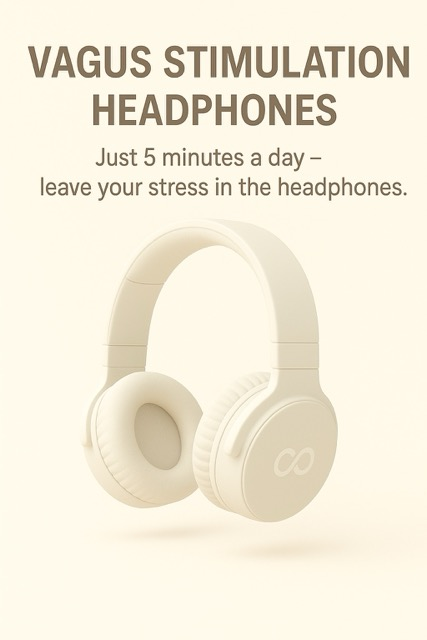
\includegraphics[keepaspectratio]{_resources/images/VNSImage Medium.jpeg}}

}

\caption{最佳VNS耳机}

\end{figure}%

正如我们在前几章中探讨的,迷走神经刺激(VNS)为压力管理、认知增强和睡眠改善提供了有前景的益处。虽然神经生理机制和临床应用已得到充分确立,但VNS技术整合到日常生活中代表着广泛采用的关键前沿。本章弥合了实验室发现与现实世界实施之间的差距,提供了将VNS纳入日常活动以实现最佳健康的框架。

\section{从临床到消费应用的转变}\label{ux4eceux4e34ux5e8aux5230ux6d88ux8d39ux5e94ux7528ux7684ux8f6cux53d8}

VNS技术从医疗干预到健康工具的演变,如第3章所述,为日常应用创造了新机会。曾经局限于癫痫和抑郁症治疗的手术植入,现在包括为日常使用设计的非侵入性、用户友好的设备。这种神经刺激技术的民主化允许个人在各种环境中获取其益处:

\begin{itemize}
\tightlist
\item
  \textbf{家庭环境}:个人设备允许进行定期刺激会话,无需临床监督
\item
  \textbf{工作场所设置}:全天的简短干预,管理压力并保持专注
\item
  \textbf{旅行场景}:便携解决方案,缓解旅行相关压力源和睡眠干扰
\item
  \textbf{运动和恢复}:与体育活动例程整合,增强表现和恢复
\end{itemize}

有效整合的关键是理解不仅是何时以及如何使用VNS,还包括如何将其无缝融入现有例程,而不增加负担或复杂性。

\section{生理准备度评估:知道何时刺激}\label{ux751fux7406ux51c6ux5907ux5ea6ux8bc4ux4f30ux77e5ux9053ux4f55ux65f6ux523aux6fc0}

在讨论具体应用之前,了解个体如何识别VNS干预可能有益的时机很重要。由于最佳VNS效果取决于当前生理状态,用户应该学会通过各种可获取的指标识别自己的自主平衡:

\subsection{自我评估技术}\label{ux81eaux6211ux8bc4ux4f30ux6280ux672f}

\begin{enumerate}
\def\labelenumi{\arabic{enumi}.}
\item
  \textbf{心率变异性意识}:最近研究表明,心率变异性(HRV)可以作为taVNS会话期间自主张力的可靠生理指标\footnote{Forte
    等 (2022)}。比较主动耳甲腔刺激与假刺激的研究发现,在时间和频域中,迷走介导的HRV参数都有显著增加。这表明用户可以通过消费可穿戴设备潜在地监测他们的HRV,以确定最佳干预时机。
\item
  \textbf{呼吸模式观察}:呼吸速率和深度提供自主状态的即时反馈。呼吸与VNS效果之间的关系是双向的------深呼吸练习可以增强VNS效果,而VNS可以改善呼吸调节。
\item
  \textbf{主观压力评分}:对感知压力的简单自评(1-10分)可以帮助用户决定何时干预最有益。这种现象学方法虽然主观,但与生理压力标记相关性相当好。
\item
  \textbf{身体紧张清单}:简短的身体扫描以识别肌肉紧张,特别是颈部、肩部和下颌,可以指示可能受益于迷走刺激的交感优势。
\end{enumerate}

Ertürk和Özden(2025)最近的比较研究表明,经皮耳迷走神经刺激和深呼吸练习在仅一次会话后就产生了感知压力量表评分、脉搏率和血压值的显著下降\footnote{Ertürk
  和 Özden (2025)}。这支持了这些简单生理测量作为VNS应用时机的反馈机制的价值。

\section{日常生活应用和使用场景}\label{ux65e5ux5e38ux751fux6d3bux5e94ux7528ux548cux4f7fux7528ux573aux666f}

基于这些评估技术,我们现在可以探索日常生活节律中的特定应用。以下场景得到了消费级VNS实施的新兴研究和用户体验数据的支持。

\subsection{晨间例程:以神经平衡开始一天}\label{ux6668ux95f4ux4f8bux7a0bux4ee5ux795eux7ecfux5e73ux8861ux5f00ux59cbux4e00ux5929}

从睡眠到清醒的过渡代表着建立一天自主张力的关键时期。研究表明,早晨HRV模式可以预测日常压力韧性和认知表现。

\textbf{实际应用:醒来调节}

\begin{itemize}
\tightlist
\item
  \textbf{时机}:醒来后立即5-10分钟
\item
  \textbf{设备放置}:使用舒适的可穿戴电极进行耳基刺激(耳甲腔)
\item
  \textbf{方案}:以3分钟低频刺激(3-5
  Hz)开始,轻轻激活副交感系统,随后5分钟中频(15-25 Hz)促进警觉性
\item
  \textbf{整合提示}:与早晨补水例程结合;在查看日程安排时使用
\end{itemize}

这一晨间方案有助于从睡眠的副交感优势过渡到日间活动的平衡交感激活,避免与突然醒来或闹钟压力相关的急剧皮质醇峰值。

\subsection{工作场所整合:认知增强和压力管理}\label{ux5de5ux4f5cux573aux6240ux6574ux5408ux8ba4ux77e5ux589eux5f3aux548cux538bux529bux7ba1ux7406}

鉴于现代工作环境的认知需求,战略性VNS应用可以支持全天的表现和福祉。

\textbf{实际应用:专注力增强}

\begin{itemize}
\tightlist
\item
  \textbf{时机}:在高浓度任务之前或注意力下滑期间(通常在上午中期和下午中期)
\item
  \textbf{设备选择}:具有谨慎形态因素的颈基或耳基刺激
\item
  \textbf{方案}:3-5分钟较高频率刺激(20-25
  Hz),激活支持注意力的蓝斑-去甲肾上腺素系统
\item
  \textbf{整合提示}:与简短工作休息配对;在重要会议或复杂任务前安排
\end{itemize}

\textbf{实际应用:压力恢复}

\begin{itemize}
\tightlist
\item
  \textbf{时机}:在压力性互动、具有挑战性的会议或强烈认知工作后
\item
  \textbf{设备选择}:带舒适耳塞的耳基刺激
\item
  \textbf{方案}:5-7分钟低频刺激(5-10 Hz)以促进副交感恢复
\item
  \textbf{整合提示}:如果可能,与简短自然暴露结合;在任务之间的过渡期使用
\end{itemize}

比较taVNS与深呼吸练习的研究表明,这些干预可以显著改变自主测量值,有利于副交感激活\footnote{Ertürk
  和 Özden (2025)}。此外,使用肌肉张力测定法测量的身体紧张度显示,即使是简短的刺激会话也能降低肌肉僵硬并增加放松------这些效果在工作场所环境中特别有价值,因为这些环境常因长时间坐姿和压力引起的肌肉紧张而特点化。

\subsection{通勤和旅行:管理过渡压力}\label{ux901aux52e4ux548cux65c5ux884cux7ba1ux7406ux8fc7ux6e21ux538bux529b}

旅行环境带来独特的压力源,包括噪音、拥挤、时间压力和例程中断。VNS可以在这些过渡期间提供稳定性。

\textbf{实际应用:通勤减压}

\begin{itemize}
\tightlist
\item
  \textbf{时机}:通勤期间或刚到家时
\item
  \textbf{设备选择}:舒适、便携的耳基刺激器
\item
  \textbf{方案}:10-15分钟交替频率(在低频和中频之间循环),促进工作和家庭心态之间的过渡
\item
  \textbf{整合提示}:在交通中与降噪功能结合;与到家时的仪式配对
\end{itemize}

对于商务旅行者,定期VNS会话可以帮助减轻与时差和日程变化相关的自主神经中断。在新时区醒来时简短的刺激可以加速昼夜节律调整。

\subsection{体育活动增强:运动前后应用}\label{ux4f53ux80b2ux6d3bux52a8ux589eux5f3aux8fd0ux52a8ux524dux540eux5e94ux7528}

运动代表对自主系统的计划性压力,VNS可以优化表现和恢复阶段。

\textbf{实际应用:运动前准备}

\begin{itemize}
\tightlist
\item
  \textbf{时机}:开始运动前5-10分钟
\item
  \textbf{设备选择}:具有运动时牢固贴合的耳基或颈基刺激
\item
  \textbf{方案}:从低频到中频(5-15
  Hz)的逐渐增加,为控制性压力准备自主系统
\item
  \textbf{整合提示}:在热身例程期间融入;与表现可视化结合
\end{itemize}

\textbf{实际应用:恢复加速}

\begin{itemize}
\tightlist
\item
  \textbf{时机}:运动后立即和/或训练日睡前
\item
  \textbf{设备选择}:为较长会话设计的舒适、固定装置
\item
  \textbf{方案}:15-20分钟主要低频(3-8 Hz)刺激以增强副交感恢复
\item
  \textbf{整合提示}:与静态伸展或休闲阅读结合;在冷静阶段使用
\end{itemize}

研究表明,在深呼吸练习和经皮VNS之间交替提供互补益处。在健康参与者和类风湿性关节炎等疾病患者的研究中,这种组合通过时域HRV参数测量显示增强的迷走张力{[}\^{}3{]}。这表明将两种模式整合到体能训练方案中可能比单独使用任一种方法提供更优越的结果。

\subsection{睡眠准备:过渡到恢复性休息}\label{ux7761ux7720ux51c6ux5907ux8fc7ux6e21ux5230ux6062ux590dux6027ux4f11ux606f}

如第6章所讨论的,VNS与睡眠质量之间的关系已得到充分建立。实际实施侧重于关键的睡前时段。

\textbf{实际应用:睡眠开始促进}

\begin{itemize}
\tightlist
\item
  \textbf{时机}:期望睡眠时间前20-30分钟
\item
  \textbf{设备选择}:舒适的耳基刺激,发光最小
\item
  \textbf{方案}:15-20分钟低频(2-5 Hz)刺激,强度逐渐降低
\item
  \textbf{整合提示}:纳入现有的就寝例程;与减少照明和避免屏幕配合
\end{itemize}

对于有入睡困难的人,这种应用可能减少对药物干预的需求。其机制似乎通过直接自主效应和入睡前减少反刍和焦虑的间接益处发挥作用。

\section{个人定制:构建你的VNS方案}\label{ux4e2aux4ebaux5b9aux5236ux6784ux5efaux4f60ux7684vnsux65b9ux6848}

虽然上述应用提供了起点,但有效整合需要基于个体反应模式、生活方式需求和生理基线的个性化。

\subsection{跟踪和调整框架}\label{ux8ddfux8e2aux548cux8c03ux6574ux6846ux67b6}

\begin{enumerate}
\def\labelenumi{\arabic{enumi}.}
\item
  \textbf{建立基线测量}:在开始定期使用VNS之前,记录压力、专注力、睡眠质量和恢复的典型模式,使用主观评级和可用的生物数据。
\item
  \textbf{从标准方案开始}:从为主要目标(减轻压力、增强专注力、改善睡眠)建立的参数开始。
\item
  \textbf{记录反应模式}:保持简单日志记录:

  \begin{itemize}
  \tightlist
  \item
    刺激前状态
  \item
    使用的方案(位置、频率、持续时间)
  \item
    刺激后立即效果
  \item
    延迟效果(几小时后)
  \end{itemize}
\item
  \textbf{迭代细化}:在7-10天后,回顾模式以识别:

  \begin{itemize}
  \tightlist
  \item
    对每个目标最有效的方案
  \item
    全天最佳时机
  \item
    最小有效刺激持续时间
  \item
    个体敏感性或副作用
  \end{itemize}
\item
  \textbf{情境适应}:根据季节变化、工作需求或健康波动调整方案。
\end{enumerate}

这种个性化方法承认VNS反应中的显著个体差异。比较耳甲腔刺激与假刺激的研究发现,虽然组级HRV增加显著,但反应幅度存在相当大的个体差异\footnote{Forte
  等 (2022)}。这强调了个性化跟踪而非依赖人群平均值的重要性。

\section{多模式整合:将VNS与互补实践结合}\label{ux591aux6a21ux5f0fux6574ux5408ux5c06vnsux4e0eux4e92ux8865ux5b9eux8df5ux7ed3ux5408}

当与其他针对类似生理系统的循证健康实践整合时,VNS的有效性可以增强。

\subsection{协同组合}\label{ux534fux540cux7ec4ux5408}

\begin{enumerate}
\def\labelenumi{\arabic{enumi}.}
\item
  \textbf{VNS +
  呼吸实践}:比较深呼吸练习和经皮VNS的研究发现,两种干预都增加副交感活动并促进肌肉放松\textsuperscript{(Ertürk
  和 Özden 2025)}(Jensen 等
  2022)。组合似乎特别有效,深呼吸在RMSSD和pNN50等副交感指标上显示更优效果,而VNS在肌肉放松测量上展示优势。
\item
  \textbf{VNS +
  温度对比}:简短冷暴露(冷水澡、面部浸泡)激活类似迷走通路。交替中等冷暴露与VNS可能增强效果。
\item
  \textbf{VNS +
  音乐/声音疗法}:具有特定频率特征的声音刺激可以增强VNS对放松和注意力的效果。一些消费设备现在提供同步声音和电刺激。
\item
  \textbf{VNS +
  光照管理}:将VNS会话与战略性光照(早晨明亮光线,睡前减少蓝光)协调可以增强昼夜节律调节。
\item
  \textbf{VNS +
  正念实践}:将taVNS与正念冥想相结合可能创造双向增强------VNS促进有利于冥想的生理状态,而冥想实践增加对迷走效应的敏感性。
\end{enumerate}

\section{技术解决方案:当前和新兴选项}\label{ux6280ux672fux89e3ux51b3ux65b9ux6848ux5f53ux524dux548cux65b0ux5174ux9009ux9879}

为支持这些应用,已经出现了多样化的VNS设备生态系统,每种设备对特定用例都有优势。如第7章所讨论的,硬件格局继续演变,目前提供了几个类别:

\subsection{关键实施考虑}\label{ux5173ux952eux5b9eux65bdux8003ux8651}

选择日常应用技术时,考虑:

\begin{enumerate}
\def\labelenumi{\arabic{enumi}.}
\tightlist
\item
  \textbf{形式因素适当性}:设备是否能舒适地融入预期使用环境?
\item
  \textbf{用户控制粒度}:系统是否提供足够的参数调整?
\item
  \textbf{反馈机制}:如何知道刺激是否有效?
\item
  \textbf{电池寿命和充电}:它是否支持您的预期使用模式?
\item
  \textbf{数据整合}:刺激会话是否可以与其他健康指标相关联?
\end{enumerate}

特别有前景的是基于实时生理监测调整刺激参数的新兴系统,创建响应全天变化条件的''闭环''调节。

\section{潜在挑战和解决方案}\label{ux6f5cux5728ux6311ux6218ux548cux89e3ux51b3ux65b9ux6848}

虽然将VNS整合到日常例程中提供显著益处,但可能出现几个常见挑战:

\subsection{依从性和一致性}\label{ux4f9dux4eceux6027ux548cux4e00ux81f4ux6027}

\textbf{挑战}:像许多健康实践一样,保持一致应用可能很困难。
\textbf{解决方案}:从最小有效方案开始;将VNS会话与现有日常锚点(早晨咖啡、通勤、就寝例程)联系起来;使用带提醒和跟踪功能的技术。

\subsection{社会接受度}\label{ux793eux4f1aux63a5ux53d7ux5ea6}

\textbf{挑战}:使用可见的神经刺激设备可能引起不必要的注意或问题。
\textbf{解决方案}:为公共场合选择谨慎的形式因素;教育亲密接触者关于目的和益处;将其框定为类似于其他健康技术。

\subsection{过度刺激风险}\label{ux8fc7ux5ea6ux523aux6fc0ux98ceux9669}

\textbf{挑战}:对益处的热情可能导致过度使用,可能降低有效性。
\textbf{解决方案}:遵循循证方案;包括''休息日''或减少刺激时段;监测减少回报。

\subsection{感觉适应}\label{ux611fux89c9ux9002ux5e94}

\textbf{挑战}:刺激的物理感觉最初可能分散注意力。
\textbf{解决方案}:从较低强度设置开始并逐渐增加;试验电极定位;将刺激与愉快活动配对以创造积极联想。

\section{结论:迈向无缝整合}\label{ux7ed3ux8bbaux8fc8ux5411ux65e0ux7f1dux6574ux5408}

随着VNS技术继续发展,目标越来越是无缝融入日常生活------神经刺激像其他健康和表现实践一样普遍。最成功的实施方法分享某些特点:

\begin{enumerate}
\def\labelenumi{\arabic{enumi}.}
\tightlist
\item
  它们与自然日常节律和过渡一致
\item
  它们补充而非竞争现有例程
\item
  它们提供引人注目的益处,强化持续使用
\item
  它们适应不断变化的需求和情境
\end{enumerate}

通过深思熟虑地应用本章概述的原则和实践,VNS可以从偶尔干预发展为日常健康的不可或缺组成部分------在我们日益苛求的世界中,为自主平衡、认知功能和压力韧性提供持续支持。

下一章将探讨VNS技术的新兴发展,包括闭环系统和AI增强方案,这些在不久的将来有望提供更精确和个性化的应用。

\bookmarksetup{startatroot}

\chapter{神经健康的未来:闭环系统和AI增强型VNS}\label{ux795eux7ecfux5065ux5eb7ux7684ux672aux6765ux95edux73afux7cfbux7edfux548caiux589eux5f3aux578bvns}

正如我们在本书中所探讨的,迷走神经刺激(VNS)已经从侵入性外科手术干预发展成为日益普及的健康工具。这项技术正在迅速发展,新兴的创新有望使VNS变得更加个性化、响应式和智能化。本章将探讨神经健康的未来发展趋势,特别关注闭环VNS系统和人工智能整合,这将彻底改变我们对心理和身体健康优化的方法。

\section{当前VNS技术的局限性}\label{ux5f53ux524dvnsux6280ux672fux7684ux5c40ux9650ux6027}

虽然今天的非侵入性VNS设备提供了显著的益处,正如前几章所讨论的,但它们仍主要作为''开环''系统运行。这意味着它们按照预先编程的参数传递刺激,而不考虑用户当前的生理或心理状态。正如第8章所探讨的,频率、强度和时机等参数可以手动调整,但真正的动态响应能力仍然有限。

这种一刀切的方法无法考虑个体对VNS的反应存在显著差异。有些用户在高压力期间可能需要更多的刺激,而其他人在某些活动中可能受益于减少刺激。VNS的有效性也因大脑状态而异,正如Rembado等人(2021)所证明的,他们发现VNS对皮质的反应会因不同的大脑状态(清醒、休息、NREM睡眠)而改变,在非人类灵长类动物中,NREM睡眠期间的反应最大\footnote{Rembado
  等 (2021)}。

\section{闭环系统:VNS技术的下一次进化}\label{ux95edux73afux7cfbux7edfvnsux6280ux672fux7684ux4e0bux4e00ux6b21ux8fdbux5316}

闭环VNS代表了当前技术的范式转变。这些先进系统不是提供固定的刺激模式,而是持续监测生理信号,并根据用户的当前状态实时调整刺激参数。

\subsection{闭环VNS的机制}\label{ux95edux73afvnsux7684ux673aux5236}

典型的闭环VNS系统由三个核心组件组成:

\begin{enumerate}
\def\labelenumi{\arabic{enumi}.}
\item
  \textbf{感知模块}:通过各种传感器收集生理数据,监测心率变异性(HRV)、皮电活动、呼吸模式,甚至通过脑电图(EEG)监测神经活动等生物标志物。O'Grady等人(2024)的最新研究验证了消费级可穿戴设备如Apple
  Watch测量HRV的准确性,使连续生理监测越来越可行\footnote{O'Grady 等
    (2024)}。
\item
  \textbf{处理单元}:分析传入数据,确定用户当前的生理和认知状态。这个组件越来越多地结合机器学习算法来检测模式并预测最佳刺激参数。
\item
  \textbf{自适应刺激模块}:根据处理单元的分析提供自动调整参数的VNS,创建一个持续优化刺激的动态反馈循环。
\end{enumerate}

这种架构允许系统响应用户内部状态的变化,仅在需要时提供刺激,并以针对最大效果而校准的参数。

\subsection{支持闭环方法的临床证据}\label{ux652fux6301ux95edux73afux65b9ux6cd5ux7684ux4e34ux5e8aux8bc1ux636e}

新兴研究证明了闭环神经调节相比传统固定参数方法的潜在优势。Toschi等人(2023)确定了经皮耳廓迷走神经刺激(taVNS)对脑干反应和心脏迷走神经输出之间的因果联系,支持以脑干为靶点的闭环刺激用于自主神经调节的可行性\footnote{Toschi
  等 (2023)}。

在癫痫研究中,研究发现基于HRV的标志物可以在发作前预测,表明VNS系统可以预先激活以预防发作。Mason等人(2024)进行的综述展示了HRV作为癫痫发作预测生物标志物的价值,强调其在闭环干预系统中的潜力\footnote{Mason
  等 (2024)}。

或许最令人信服的是Fang等人(2021)的工作,他们开发了一个机器学习模型,使用术前HRV指标来预测难治性癫痫患者的VNS治疗结果。他们的模型在预测哪些患者会对VNS治疗产生反应方面达到了74.6\%的准确率,展示了生理生物标志物如何能够为个性化治疗方法提供信息\footnote{Fang
  等 (2021)}。

\section{人工智能:先进VNS系统的大脑}\label{ux4ebaux5de5ux667aux80fdux5148ux8fdbvnsux7cfbux7edfux7684ux5927ux8111}

神经健康领域的真正革命将来自人工智能与VNS技术的整合。AI系统可以检测人类可能错过的生理数据中的微妙模式,预测最佳刺激参数,并从用户反应中不断学习以提高效果。

\subsection{机器学习用于模式识别}\label{ux673aux5668ux5b66ux4e60ux7528ux4e8eux6a21ux5f0fux8bc6ux522b}

机器学习算法可以通过分析跨用户的大量数据,识别生理状态和最佳VNS参数之间的相关性。例如,AI系统可能了解到特定的HRV波动模式在10Hz而非25Hz的刺激下反应最佳,或者在特定睡眠阶段进行刺激对特定情况产生更好的结果。

Ding等人(2019)展示了如何使用生理数据(EEG、眼动追踪和皮电反应)的机器学习方法成功地以79.63\%的准确率区分抑郁症患者和健康对照组\footnote{Ding
  等 (2019)}。类似的方法可能用于根据检测到的心理状态校准VNS参数。

\subsection{个性化参数优化}\label{ux4e2aux6027ux5316ux53c2ux6570ux4f18ux5316}

除了模式识别外,AI系统还可以开发个性化的用户模型,考虑他们独特的生理状况和反应模式。这些模型使得真正个性化的刺激方案成为可能,随着系统对用户了解的加深而不断发展。

Bolz和Bolz(2022)讨论了利用设备和受试者数据优化VNS参数的进化算法的潜力,表明个性化的tVNS治疗可能显著改善结果\footnote{Bolz
  和 Bolz (2022)}。这种自适应方法比第8章中描述的手动参数调整代表了实质性的进步。

\subsection{AI驱动的配套应用}\label{aiux9a71ux52a8ux7684ux914dux5957ux5e94ux7528}

AI的整合不仅限于刺激设备本身,还扩展到增强整体用户体验的配套应用:

\begin{itemize}
\tightlist
\item
  \textbf{虚拟教练}:提供有效使用VNS的指导并将其与其他健康实践相结合的AI系统
\item
  \textbf{预测分析}:在影响用户之前识别潜在触发因素或压力源的工具
\item
  \textbf{进展跟踪}:对目标条件改善的复杂分析
\end{itemize}

Siddals、Torous和Coxon(2024)的最新研究探索了AI聊天机器人如何为用户提供有意义的心理健康支持\textsuperscript{(Siddals,
Torous, 和 Coxon
2024),而Raile(2024)则研究了ChatGPT对心理治疗师和患者的实用性}(Raile
2024)。这些研究表明,AI伴侣可以通过在生理干预的同时提供心理支持,增强VNS的治疗价值。

\section{生物标志物创新:超越传统测量}\label{ux751fux7269ux6807ux5fd7ux7269ux521bux65b0ux8d85ux8d8aux4f20ux7edfux6d4bux91cf}

闭环VNS系统的有效性很大程度上取决于能够准确反映用户状态的相关生物标志物。未来的系统可能会整合多个生物标志物,以创建对生理和心理状况的全面理解。

\subsection{新型生理标志物}\label{ux65b0ux578bux751fux7406ux6807ux5fd7ux7269}

除了已经建立的测量方法如HRV外,研究人员正在探索可能提供更深入神经状态洞察的额外生物标志物:

\begin{itemize}
\tightlist
\item
  \textbf{瞳孔测量}:Sharon等人(2021)证明taVNS会导致瞳孔扩张并减弱α波振荡,表明瞳孔反应可作为taVNS效果的潜在生物标志物\footnote{Sharon,
    Fahoum, 和 Nir (2021)}。
\item
  \textbf{脑电图同步}:Danthine等人(2024)探讨了脑电图同步测量作为难治性癫痫VNS反应的潜在预测生物标志物\footnote{Danthine,
    V., Cottin, L., Berger, A., Morrison, E. I. G., Liberati, G.,
    Santos, S. F., Delbeke, J., Nonclercq, A., \& El Tahry, R. (2024).
    Electroencephalogram synchronization measure as a predictive
    biomarker of Vagus nerve stimulation response in refractory
    epilepsy: A retrospective study. PLOS ONE, 19(6), e0304115.}。
\item
  \textbf{视网膜生物标志物}:Constable、Lim和Thompson(2023)回顾了视网膜电生理如何作为中枢神经系统疾病的''大脑窗口''\footnote{Constable,
    P. A., Lim, J. K. H., \& Thompson, D. A. (2023). Retinal
    electrophysiology in central nervous system disorders. A review of
    human and mouse studies. Frontiers in Neuroscience, 17, 1215097.}。
\end{itemize}

Pervaz等人(2025)进行了贝叶斯元分析,探索不同taVNS协议对瞳孔扩张的影响,发现脉冲刺激协议比持续刺激在诱导瞳孔变化方面显著更有效\footnote{Pervaz,
  I., Thurn, L., Vezzani, C., Kaluza, L., Kühnel, A., \& Kroemer, N. B.
  (2025). Does transcutaneous auricular vagus nerve stimulation alter
  pupil dilation? A living Bayesian meta-analysis. Brain Stimulation,
  18(2), 148-157.}。这类研究有助于识别哪些生物标志物最可靠地反映不同刺激方法的效果。

\subsection{多模态感知}\label{ux591aux6a21ux6001ux611fux77e5}

未来的VNS系统可能会结合多种感知模式,创建用户状态的更全面图景。例如,系统可能同时监测HRV、呼吸模式、皮肤电导率,甚至通过嵌入在日常可穿戴设备中的紧凑型脑电图传感器监测神经活动。

多个传感器的整合使更细微的状态检测成为可能,并减少了响应确定中假阳性或假阴性的可能性。例如,Ertürk和Özden(2025)比较了taVNS和深呼吸练习对自主神经系统活动的急性影响,证明多种生理测量提供了干预效果的互补洞察\footnote{Ertürk,
  Ç., \& Özden, A. V. (2025). Comparison of the Acute Effects of
  Auricular Vagus Nerve Stimulation and Deep Breathing Exercise on the
  Autonomic Nervous System Activity and Biomechanical Properties of the
  Muscle in Healthy People. Journal of Clinical Medicine, 14(4), 1046.}。

\section{实用应用和形态因素}\label{ux5b9eux7528ux5e94ux7528ux548cux5f62ux6001ux56e0ux7d20}

闭环技术和AI的结合将使VNS的全新应用和形态成为可能,使神经健康更加融入日常生活。

\subsection{下一代可穿戴设备}\label{ux4e0bux4e00ux4ee3ux53efux7a7fux6234ux8bbeux5907}

未来的VNS设备将变得越来越隐蔽和舒适,可能采取以下形式:

\begin{itemize}
\tightlist
\item
  \textbf{先进耳塞}:基于当前的耳戴和入耳式设计,未来设备可能将感知和刺激功能整合到与标准无线耳机无法区分的耳塞形态中。
\item
  \textbf{智能珠宝}:戒指、项链或手环提供持续监测和刺激,无明显医疗美学。
\item
  \textbf{隐形可穿戴设备}:超薄、粘贴式贴片,甚至类似临时纹身的界面,直接附着在刺激点上。
\end{itemize}

正如我们所考察的产品材料所证明的,制造商已经朝着更加注重美学和舒适度的消费者友好设计迈进。这些形态因素的发展对于神经健康技术的主流采用至关重要。

\subsection{与智能环境的整合}\label{ux4e0eux667aux80fdux73afux5883ux7684ux6574ux5408}

除了可穿戴设备,VNS技术最终可能与智能家居和工作场所整合,创建支持神经健康的环境:

\begin{itemize}
\tightlist
\item
  \textbf{环境感知}:检测压力指标并触发适当刺激的环境系统
\item
  \textbf{多设备协调}:VNS与照明、声音和其他环境因素的同步
\item
  \textbf{情境感知干预}:了解用户当前活动并相应优化刺激的系统
\end{itemize}

这种级别的整合将把VNS从离散干预转变为神经优化的连续、环境支持系统。

\section{伦理考虑和挑战}\label{ux4f26ux7406ux8003ux8651ux548cux6311ux6218}

与任何影响人类认知和生理的先进技术一样,下一代VNS系统引发了必须解决的重要伦理问题:

\subsection{数据隐私和安全}\label{ux6570ux636eux9690ux79c1ux548cux5b89ux5168}

闭环系统所需的广泛生理监测带来了显著的隐私问题。用户的神经和生理数据代表高度敏感的信息,可能揭示有关其心理和身体健康、情绪状态甚至决策过程的详细洞察。

随着这些技术的发展,防止未经授权的访问并建立明确的数据所有权和使用协议至关重要。用户必须保持对其神经数据的控制,并了解它如何被用于优化他们的体验。

\subsection{自主性和能动性}\label{ux81eaux4e3bux6027ux548cux80fdux52a8ux6027}

随着AI系统承担更大的刺激参数确定责任,关于用户自主权的问题出现了。用户在多大程度上应该能够覆盖AI建议?系统如何平衡自动化与用户控制?

Mitsea、Drigas和Skianis(2023)探索了智能技术支持的数字辅助正念干预如何有效帮助发展自我调节技能,同时保持用户能动性\footnote{Mitsea,
  E., Drigas, A., \& Skianis, C. (2023). Digitally Assisted Mindfulness
  in Training Self-Regulation Skills for Sustainable Mental Health: A
  Systematic Review. Behavioral Sciences, 13(12), 1008.}。类似的原则需要应用于AI增强型VNS系统。

\subsection{可及性和公平性}\label{ux53efux53caux6027ux548cux516cux5e73ux6027}

最先进的神经健康技术最初可能价格高昂,可能导致获取不平等。确保这些潜在变革性技术不会加剧现有健康不平等,需要在定价、分销甚至政策方面采取深思熟虑的方法。

正如我们在第7章所见,即使当前的消费级VNS设备价格也差异显著,高端选项对许多可能从中受益的潜在用户来说仍然遥不可及。

\section{前进道路:跨学科合作}\label{ux524dux8fdbux9053ux8defux8de8ux5b66ux79d1ux5408ux4f5c}

实现闭环、AI增强型VNS的全部潜力需要前所未有的跨学科合作:

\subsection{神经科学与工程合作}\label{ux795eux7ecfux79d1ux5b66ux4e0eux5de5ux7a0bux5408ux4f5c}

持续进步需要了解迷走神经复杂功能的神经科学家与开发有效界面技术的工程师之间的深度合作。这些学科的整合已经推动了重大创新,正如Wang等人(2024)回顾VNS效率和对认知功能作用机制的进展所见\footnote{Wang,
  W., Li, R., Li, C., Liang, Q., \& Gao, X. (2024). Advances in VNS
  efficiency and mechanisms of action on cognitive functions. Frontiers
  in Physiology, 15, 1452490.}。

\subsection{临床验证}\label{ux4e34ux5e8aux9a8cux8bc1}

随着新技术的出现,严格的临床验证对于确立有效性、安全性和最佳用例至关重要。Wu等人(2022)对原发性失眠taVNS有效性的随机对照试验\footnote{Wu,
  Y., Song, L., Wang, X., Li, N., Zhan, S., Rong, P., Wang, Y., \& Liu,
  A. (2022). Transcutaneous Vagus Nerve Stimulation Could Improve the
  Effective Rate on the Quality of Sleep in the Treatment of Primary
  Insomnia: A Randomized Control Trial. Brain Sciences, 12(10), 1296.}和Xu等人(2025)对癫痫患者抑郁症的研究\footnote{Xu,
  Z. Y. R., Fang, J. J., Fan, X. Q., Xu, L. L., Jin, G. F., Lei, M. H.,
  Wang, Y. F., Liu, J. B., Dong, F., Jiang, L. R., \& Guo, Y. (2025).
  Effectiveness and safety of transcutaneous auricular vagus nerve
  stimulation for depression in patients with epilepsy. Epilepsy \&
  Behavior, 163, 110226.}提供了未来技术验证的模型。

\subsection{以用户为中心的设计}\label{ux4ee5ux7528ux6237ux4e3aux4e2dux5fc3ux7684ux8bbeux8ba1}

或许最重要的是,推进神经健康技术需要与用户深入互动,了解他们的需求、偏好和体验。正如Winter等人(2024)探索VNS用于发作性睡病的应用\footnote{Winter,
  Y., Sandner, K., Bassetti, C. L. A., Glaser, M., Ciolac, D., Ziebart,
  A., Karakoyun, A., Saryyeva, A., Krauss, J. K., Ringel, F., \& Groppa,
  S. (2024). Vagus nerve stimulation for the treatment of narcolepsy.
  Brain Stimulation, 17(1), 83-88.}和Yang等人(2024)为系统评估taVNS治疗失眠制定协议\footnote{Yang,
  T., Cai, Y., Li, X., Fang, L., \& Hu, H. (2024). Is transcutaneous
  auricular vagus nerve stimulation effective and safe for primary
  insomnia? A PRISMA-compliant protocol for a systematic review and
  meta-analysis. PLOS ONE, 19(11), e0313101.},用户体验必须指导技术发展。

\section{结论:个性化神经健康的未来}\label{ux7ed3ux8bbaux4e2aux6027ux5316ux795eux7ecfux5065ux5eb7ux7684ux672aux6765}

通过VNS技术的神经健康未来有望从标准化干预转向高度个性化、响应式系统,实时适应个体需求。由人工智能增强的闭环系统将改变我们理解和优化自身神经功能的方式,可能以前所未有的精确度解决从焦虑和抑郁到认知表现和睡眠障碍的各种状况。

当我们站在这个新时代的门槛上,先进感知、人工智能和迷走神经刺激的整合不仅代表技术演进,也代表我们如何看待心理和身体健康的根本性重新构想。通过与我们的神经系统合作而不仅仅是处理其症状,这些技术展现了未来的愿景,神经健康将成为日常生活的一部分,像今天的体育锻炼一样普及和例行。

明天的迷走神经优势不仅仅是我们使用的技术,而是理解并响应我们神经需求的智能系统------在追求最佳健康和表现的道路上的真正伙伴。

\bookmarksetup{startatroot}

\chapter{总结与结论}\label{ux603bux7ed3ux4e0eux7ed3ux8bba}

随着我们探索的旅程接近尾声,现在是时候回顾我们所涵盖的关键主题,并展望迷走神经刺激(VNS)作为神经调节工具的未来发展方向。本书的主要目标是弥合科学理解与实际应用之间的鸿沟,为读者提供既有科学依据又有实用性的知识基础。在这最后的章节中,我们将综合前面各章的洞见,为希望将VNS整合到他们的健康实践、临床工作或研究项目中的读者总结核心要点。

\section{迷走神经刺激:从理论到实践的转变}\label{ux8ff7ux8d70ux795eux7ecfux523aux6fc0ux4eceux7406ux8bbaux5230ux5b9eux8df5ux7684ux8f6cux53d8}

我们的探索始于理解迷走神经的基础解剖结构和功能------这条''神经高速公路''以其广泛的身体内部连接和对多种生理系统的调节作用而独树一帜。迷走神经的双向特性------既将信息从大脑传递到身体,又从身体返回到大脑------使其成为神经调节的理想目标。这种结构基础为所有后续章节中讨论的临床和健康应用提供了支撑。

在神经科学层面,VNS展示了复杂而广泛的作用机制。我们探讨了它如何通过NTS-LC通路促进去甲肾上腺素释放,通过下调交感神经活动和增强副交感神经张力改变自主神经平衡,通过调节炎症反射降低全身炎症,以及通过增强神经元振荡的同步性促进大脑网络功能。这些机制不仅解释了VNS的多样化效应,也使我们能够更具策略性地应用这项技术,针对特定结果选择最佳刺激参数。

这一科学基础支持了VNS从严格医疗用途向广泛健康应用的转变。从最初作为难治性癫痫的手术治疗开始,VNS已经演变成各种非侵入性形式,从处方器械到消费者友好的健康工具。这一转变代表了更广泛的趋势,即神经调节从临床病理学向日常健康优化的拓展。

\section{关键应用领域的证据总结}\label{ux5173ux952eux5e94ux7528ux9886ux57dfux7684ux8bc1ux636eux603bux7ed3}

纵观全书,我们深入探讨了VNS在三个主要领域的应用,每个领域的证据基础都在不断扩大:

\subsection{压力管理与情绪调节}\label{ux538bux529bux7ba1ux7406ux4e0eux60c5ux7eeaux8c03ux8282}

正如第4章所详述,VNS对自主神经系统的调节作用使其成为压力和焦虑管理的有力工具。研究表明,VNS可以:

\begin{itemize}
\tightlist
\item
  抑制皮质醇等压力激素的释放
\item
  增加代表副交感神经活动的心率变异性(HRV)指标
\item
  通过减少促炎性细胞因子降低与压力相关的炎症
\item
  降低经历焦虑障碍的个体的主观症状和生理激活
\end{itemize}

非侵入性VNS,特别是经皮耳廓VNS(taVNS),已被证明在急性压力反应中具有显著的缓解作用,在长期应用时可能降低基线焦虑水平。这一领域的证据支持将VNS作为传统药物和心理治疗方法的补充,为那些寻求避免药物副作用的人提供了令人鼓舞的选择。

\subsection{认知能力与注意力}\label{ux8ba4ux77e5ux80fdux529bux4e0eux6ce8ux610fux529b}

第5章探讨了VNS对大脑认知网络的强化作用。通过激活LC-NE通路,VNS已被证明能够:

\begin{itemize}
\tightlist
\item
  提高注意力聚焦能力和警觉性
\item
  增强工作记忆性能和信息处理速度
\item
  促进神经可塑性,支持更有效的学习和记忆形成
\item
  在疲劳和压力状态下维持认知表现
\end{itemize}

这些效果与Robert
Desimone博士和其他研究者描述的神经同步现象相符,在这一现象中,成功的注意力聚焦涉及神经元的协调发放------``像合唱团一样从噪音中脱颖而出''。VNS通过促进这种同步,帮助增强信号与噪音的比例,提高认知效率。

\subsection{睡眠质量与恢复}\label{ux7761ux7720ux8d28ux91cfux4e0eux6062ux590d}

第6章详细阐述了VNS在支持健康睡眠和恢复过程中的应用。证据表明,VNS可以:

\begin{itemize}
\tightlist
\item
  缩短入睡时间和减少夜间觉醒
\item
  增加深度慢波睡眠占比
\item
  改善睡眠架构和睡眠质量的主观评分
\item
  加强睡眠与清醒转换期的自主神经调节
\end{itemize}

对原发性失眠患者的随机对照试验已表明taVNS能显著改善睡眠参数。这一领域特别有希望,因为睡眠障碍与多种健康问题相关,而现有的药物治疗往往带来依赖性和其他副作用。

\section{技术考量与实施指南}\label{ux6280ux672fux8003ux91cfux4e0eux5b9eux65bdux6307ux5357}

为了使VNS的理论应用转化为实际实践,我们详细探讨了与设备选择、参数优化和日常整合相关的关键考虑因素。

\subsection{设备选择}\label{ux8bbeux5907ux9009ux62e9}

第7章比较了各种VNS技术平台,帮助读者在多样化的选择中进行导航。核心考虑因素包括:

\begin{itemize}
\tightlist
\item
  \textbf{基于耳朵vs颈部的刺激}:耳廓分支VNS提供便捷性和不引人注目的特点,而颈部刺激可能提供更直接的主要迷走神经干刺激
\item
  \textbf{刺激强度与深度}:医疗级设备通常提供更强的刺激能力,而消费级设备优先考虑舒适度
\item
  \textbf{可用性与便携性}:颈戴式、耳机式和手持式设备提供不同程度的便携性和易用性
\item
  \textbf{价格与可及性}:从数百到数千美元不等,反映了功能复杂程度和验证程度的差异
\end{itemize}

随着VNS市场的成熟,这些设备类别之间的界限正在模糊,促进了更符合人体工程学、功能更强大的设计的出现。

\subsection{参数优化与个性化}\label{ux53c2ux6570ux4f18ux5316ux4e0eux4e2aux6027ux5316}

第8章深入探讨了刺激参数的关键性,这些参数决定了VNS的效果和耐受性。核心参数包括:

\begin{itemize}
\tightlist
\item
  \textbf{频率}:高频(20-30 Hz)可能优先促进认知和注意力效果,而低频(1-10
  Hz)更侧重于放松和自主神经平衡
\item
  \textbf{强度}:有效剂量必须平衡最大效果与舒适度和安全性
\item
  \textbf{波形}:从简单的双相脉冲到复杂的载波调制波形,不同设计针对不同目标
\item
  \textbf{时长与占空比}:确定刺激的总量和分布,影响效果持久性和耐受性
\end{itemize}

随着用户收集个人数据并记录其反应,参数可以精细调整以创建高度个性化的方案。这种方法认识到个体对VNS反应存在显著差异,避免了''一刀切''的局限性。

\subsection{实际应用场景}\label{ux5b9eux9645ux5e94ux7528ux573aux666f}

第9章将VNS的应用扩展到日常生活环境中,提供了实际实施指南。建议的应用场景包括:

\begin{itemize}
\tightlist
\item
  \textbf{早晨唤醒}:利用VNS快速激活注意力网络,有效开始一天
\item
  \textbf{工作增强}:在高要求认知任务前或期间的短暂刺激可提高注意力和工作表现
\item
  \textbf{压力恢复}:在压力事件后使用VNS加速副交感神经恢复
\item
  \textbf{旅行和通勤}:通过便携式刺激帮助管理旅行相关的压力和疲劳
\item
  \textbf{睡前过渡}:晚间VNS可以促进从交感主导的清醒状态转向副交感主导的睡眠状态
\end{itemize}

这些场景利用了特定参数组合以最大化特定情境中的益处,同时提供简单的使用者流程,使VNS成为日常生活的无缝组成部分。

\section{未来方向:神经健康的新范式}\label{ux672aux6765ux65b9ux5411ux795eux7ecfux5065ux5eb7ux7684ux65b0ux8303ux5f0f}

展望未来,VNS技术有望继续发展,呈现出几个令人兴奋的趋势:

\subsection{闭环系统}\label{ux95edux73afux7cfbux7edf}

第10章探讨了闭环系统的兴起,这些系统不仅提供刺激,还实时监测生理反应,动态调整参数。这些系统可以:

\begin{itemize}
\tightlist
\item
  根据实时HRV测量调整强度和频率
\item
  利用呼吸和皮电活动等多种生物标志物评估用户状态
\item
  预测最佳干预时机,而不是仅在症状出现后才做出反应
\item
  学习个人反应模式,随着时间推移提高准确性
\end{itemize}

闭环方法代表了从''一次性''刺激向动态个性化神经调节的重要转变。

\subsection{AI辅助优化}\label{aiux8f85ux52a9ux4f18ux5316}

人工智能和机器学习的整合正在彻底改变VNS的个性化方式:

\begin{itemize}
\tightlist
\item
  分析大规模用户数据集以识别最佳参数组合
\item
  建立预测性个体模型,考虑生理、环境和行为因素
\item
  为特定应用场景创建自定义刺激方案
\item
  将VNS数据与其他健康指标相关联,以全面了解效果
\end{itemize}

这些技术跨越了健康科技和神经科学之间的鸿沟,使更智能、更细致入微的干预成为可能。

\subsection{多模态健康整合}\label{ux591aux6a21ux6001ux5065ux5eb7ux6574ux5408}

VNS不太可能作为单一干预措施提供最佳结果;相反,它会融入更全面的健康实践中:

\begin{itemize}
\tightlist
\item
  与呼吸练习和正念冥想等传统实践的协同作用
\item
  通过可穿戴生态系统整合营养、运动和睡眠数据
\item
  使用指导应用程序提供教育和练习,使VNS成为更广泛健康策略的组成部分
\item
  有针对性的干预措施,解决特定健康和绩效目标
\end{itemize}

这种整合方式避免了技术孤立的局限性,而是将神经调节视为整体健康的关键组成部分。

\section{平衡乐观与现实:VNS的局限性与挑战}\label{ux5e73ux8861ux4e50ux89c2ux4e0eux73b0ux5b9evnsux7684ux5c40ux9650ux6027ux4e0eux6311ux6218}

尽管本书关注VNS的潜力和益处,但我们必须承认这一领域仍面临重要的局限性和挑战:

\subsection{研究的局限性}\label{ux7814ux7a76ux7684ux5c40ux9650ux6027}

尽管VNS的证据基础日益壮大,但仍存在显著的知识差距:

\begin{itemize}
\tightlist
\item
  许多研究使用小样本,可能夸大效果或忽视小子群体的差异
\item
  参数与效果的关系尚未完全映射,导致方案选择常基于经验而非确证
\item
  长期使用的成果数据有限,需要更多研究以确立持久益处
\item
  消费级设备常缺乏与医疗级应用相同水平的严格评估
\end{itemize}

\subsection{个体变异性}\label{ux4e2aux4f53ux53d8ux5f02ux6027}

对VNS的反应表现出显著的个体差异,可能受多种因素影响:

\begin{itemize}
\tightlist
\item
  迷走神经解剖学和分支模式的个体变异
\item
  基线自主神经功能差异
\item
  年龄、性别和健康状况的影响
\item
  并发药物和健康实践的相互作用
\end{itemize}

这种变异性意味着VNS永远不会是''一刀切''的解决方案,而是需要个性化和调整。

\subsection{技术和可及性挑战}\label{ux6280ux672fux548cux53efux53caux6027ux6311ux6218}

随着VNS技术的发展,仍存在重要障碍:

\begin{itemize}
\tightlist
\item
  高效设备的成本可能限制获取和使用
\item
  调整参数需要一定程度的技术理解,可能对一些用户构成障碍
\item
  设备耐久性和电池寿命可能限制实际使用
\item
  技术支持和长期维护对持续使用至关重要
\end{itemize}

\subsection{伦理考量}\label{ux4f26ux7406ux8003ux91cf}

随着神经调节技术的普及,出现了重要的伦理问题:

\begin{itemize}
\tightlist
\item
  数据隐私和安全关切,特别是涉及神经和生理数据
\item
  获取和教育的公平性,避免''神经健康鸿沟''的扩大
\item
  避免替代解决根本问题所需的更广泛社会变革的''技术修复''心态
\item
  确保用户了解与神经调节相关的潜在风险和局限
\end{itemize}

\section{结论:迈向神经健康未来的平衡方法}\label{ux7ed3ux8bbaux8fc8ux5411ux795eux7ecfux5065ux5eb7ux672aux6765ux7684ux5e73ux8861ux65b9ux6cd5}

总的来说,VNS有潜力成为我们健康工具箱中的重要补充,尤其是在管理压力、提升认知表现和促进恢复方面。它提供了一种独特的接触点,允许我们以非侵入性方式影响复杂的神经网络。然而,最大的益处可能来自将VNS作为更全面健康战略的一部分,而不是孤立的''神奇解决方案''。

通过科学基础和实际应用的双重视角审视VNS,我们可以超越炒作和怀疑,采取更细微的立场。对于专业人士,VNS提供了一种补充传统干预的工具;对于研究人员,它开辟了关于神经调节的新问题;对于个人,它提供了积极参与自身神经调节的机会。

随着科技继续发展,神经调节很可能成为日常健康实践中越来越普遍的一部分。那些了解这一领域基本科学并能明智地应用这些知识的人将处于有利位置,能够从这一令人兴奋的新范式中受益------在这一范式中,我们可以直接与连接大脑和身体的神经通路''对话'',促进最佳的身心健康。

``迷走神经优势''不仅仅是使用特定技术的能力,而是理解并有意识地影响神经系统的内在调节能力,从而在日益复杂和充满压力的世界中培养复原力、专注力和平静。通过平衡创新的兴奋与科学的严谨,我们可以负责任地利用这些新兴技术,不仅处理症状,还解决更深层次的生理调节,使我们所有人受益。

\bookmarksetup{startatroot}

\chapter*{参考文献}\label{ux53c2ux8003ux6587ux732e}
\addcontentsline{toc}{chapter}{参考文献}

\markboth{参考文献}{参考文献}

\phantomsection\label{refs}
\begin{CSLReferences}{1}{0}
\bibitem[\citeproctext]{ref-addorisioInvestigationalTreatmentRheumatoid2019}
Addorisio, Meghan E., Gavin H. Imperato, Alex F. De Vos, Steve Forti,
Richard S. Goldstein, Valentin A. Pavlov, Tom Van Der Poll, 等. 2019.
{《Investigational Treatment of Rheumatoid Arthritis with a Vibrotactile
Device Applied to the External Ear》}. \emph{Bioelectronic Medicine} 5
(1): 4. \url{https://doi.org/10.1186/s42234-019-0020-4}.

\bibitem[\citeproctext]{ref-alkhawajahImpactAutonomicNervous2024}
Alkhawajah, Hani A., Ali M. Y. Alshami, 和 Ali M. Albarrati. 2024.
{《The {Impact} of {Autonomic Nervous System Modulation} on {Heart Rate
Variability} and {Musculoskeletal Manifestations} in {Chronic Neck
Pain}: {A Double-Blind Randomized Clinical Trial}》}. \emph{Journal of
Clinical Medicine} 14 (1): 153.
\url{https://doi.org/10.3390/jcm14010153}.

\bibitem[\citeproctext]{ref-badranNeurophysiologicEffectsTranscutaneous2018}
Badran, Bashar W., Logan T. Dowdle, Oliver J. Mithoefer, Nicholas T.
LaBate, James Coatsworth, Joshua C. Brown, William H. DeVries,
Christopher W. Austelle, Lisa M. McTeague, 和 Mark S. George. 2018.
{《Neurophysiologic Effects of Transcutaneous Auricular Vagus Nerve
Stimulation ({taVNS}) via Electrical Stimulation of the Tragus: {A}
Concurrent {taVNS}/{fMRI} Study and Review》}. \emph{Brain Stimulation}
11 (3): 492--500. \url{https://doi.org/10.1016/j.brs.2017.12.009}.

\bibitem[\citeproctext]{ref-bolzTechnicalAspectsFuture2022}
Bolz, Armin, 和 Lars-Oliver Bolz. 2022. {《Technical Aspects and Future
Approaches in Transcutaneous Vagus Nerve Stimulation ({tVNS})》}.
\emph{Autonomic Neuroscience} 239 (五月): 102956.
\url{https://doi.org/10.1016/j.autneu.2022.102956}.

\bibitem[\citeproctext]{ref-bremnerApplicationNoninvasiveVagal2020}
Bremner, James Douglas, Nil Z. Gurel, Matthew T. Wittbrodt, Mobashir H.
Shandhi, Mark H. Rapaport, Jonathon A. Nye, Bradley D. Pearce, 等. 2020.
{《Application of {Noninvasive Vagal Nerve Stimulation} to
{Stress-Related Psychiatric Disorders}》}. \emph{Journal of Personalized
Medicine} 10 (3): 119. \url{https://doi.org/10.3390/jpm10030119}.

\bibitem[\citeproctext]{ref-bublSeeingGrayWhen2010}
Bubl, Emanuel, Elena Kern, Dieter Ebert, Michael Bach, 和 Ludger Tebartz
Van Elst. 2010. {《Seeing {Gray When Feeling Blue}? {Depression Can Be
Measured} in the {Eye} of the {Diseased}》}. \emph{Biological
Psychiatry} 68 (2): 205--8.
\url{https://doi.org/10.1016/j.biopsych.2010.02.009}.

\bibitem[\citeproctext]{ref-canliAmygdalaReactivityEmotional2005}
Canli, Turhan, Rebecca E. Cooney, Philippe Goldin, Maulik Shah, Heidi
Sivers, Moriah E. Thomason, Susan Whitfield-Gabrieli, John D. E.
Gabrieli, 和 Ian H. Gotlib. 2005. {《Amygdala Reactivity to Emotional
Faces Predicts Improvement in Major Depression》}. \emph{NeuroReport} 16
(12): 1267--70.
\url{https://doi.org/10.1097/01.wnr.0000174407.09515.cc}.

\bibitem[\citeproctext]{ref-canliBrainActivationEmotional2004}
Canli, Turhan, Heidi Sivers, Moriah E. Thomason, Susan
Whitfield-Gabrieli, John D. E. Gabrieli, 和 Ian H. Gotlib. 2004.
{《Brain Activation to Emotional Words in Depressed Vs Healthy
Subjects:》} \emph{NeuroReport} 15 (17): 2585--88.
\url{https://doi.org/10.1097/00001756-200412030-00005}.

\bibitem[\citeproctext]{ref-caoAccuracyAssessmentOura2022}
Cao, Rui, Iman Azimi, Fatemeh Sarhaddi, Hannakaisa Niela-Vilen, Anna
Axelin, Pasi Liljeberg, 和 Amir M Rahmani. 2022. {《Accuracy
{Assessment} of {Oura Ring Nocturnal Heart Rate} and {Heart Rate
Variability} in {Comparison With Electrocardiography} in {Time} and
{Frequency Domains}: {Comprehensive Analysis}》}. \emph{Journal of
Medical Internet Research} 24 (1): e27487.
\url{https://doi.org/10.2196/27487}.

\bibitem[\citeproctext]{ref-capilupiVagusNerveStimulation2020}
Capilupi, Michael J., Samantha M. Kerath, 和 Lance B. Becker. 2020.
{《Vagus {Nerve Stimulation} and the {Cardiovascular System}》}.
\emph{Cold Spring Harbor Perspectives in Medicine} 10 (2): a034173.
\url{https://doi.org/10.1101/cshperspect.a034173}.

\bibitem[\citeproctext]{ref-chaiFunctionalStructuralBrain2015}
Chai, Xiaoqian J., Dina Hirshfeld-Becker, Joseph Biederman, Mai Uchida,
Oliver Doehrmann, Julia A. Leonard, John Salvatore, 等. 2015.
{《Functional and Structural Brain Correlates of Risk for Major
Depression in Children with Familial Depression》}. \emph{NeuroImage:
Clinical} 8: 398--407. \url{https://doi.org/10.1016/j.nicl.2015.05.004}.

\bibitem[\citeproctext]{ref-constableRetinalElectrophysiologyCentral2023}
Constable, Paul A., Jeremiah K. H. Lim, 和 Dorothy A. Thompson. 2023.
{《Retinal Electrophysiology in Central Nervous System Disorders. {A}
Review of Human and Mouse Studies》}. \emph{Frontiers in Neuroscience}
17 (八月): 1215097. \url{https://doi.org/10.3389/fnins.2023.1215097}.

\bibitem[\citeproctext]{ref-danthineElectroencephalogramSynchronizationMeasure2024}
Danthine, Venethia, Lise Cottin, Alexandre Berger, Enrique Ignacio
Germany Morrison, Giulia Liberati, Susana Ferrao Santos, Jean Delbeke,
Antoine Nonclercq, 和 Riëm El Tahry. 2024. {《Electroencephalogram
Synchronization Measure as a Predictive Biomarker of {Vagus} Nerve
Stimulation Response in Refractory Epilepsy: {A} Retrospective Study》}.
编辑 Ayataka Fujimoto. \emph{PLOS ONE} 19 (6): e0304115.
\url{https://doi.org/10.1371/journal.pone.0304115}.

\bibitem[\citeproctext]{ref-dingClassifyingMajorDepression2019}
Ding, Xinfang, Xinxin Yue, Rui Zheng, Cheng Bi, Dai Li, 和 Guizhong Yao.
2019. {《Classifying Major Depression Patients and Healthy Controls
Using {EEG}, Eye Tracking and Galvanic Skin Response Data》}.
\emph{Journal of Affective Disorders} 251 (五月): 156--61.
\url{https://doi.org/10.1016/j.jad.2019.03.058}.

\bibitem[\citeproctext]{ref-erturkComparisonAcuteEffects2025}
Ertürk, Çağıl, 和 Ali Veysel Özden. 2025. {《Comparison of the {Acute
Effects} of {Auricular Vagus Nerve Stimulation} and {Deep Breathing
Exercise} on the {Autonomic Nervous System Activity} and {Biomechanical
Properties} of the {Muscle} in {Healthy People}》}. \emph{Journal of
Clinical Medicine} 14 (4): 1046.
\url{https://doi.org/10.3390/jcm14041046}.

\bibitem[\citeproctext]{ref-fangPreoperativeHeartRate2021}
Fang, Xi, Hong-Yun Liu, Zhi-Yan Wang, Zhao Yang, Tung-Yang Cheng,
Chun-Hua Hu, Hong-Wei Hao, 等. 2021. {《Preoperative {Heart Rate
Variability During Sleep Predicts Vagus Nerve Stimulation Outcome
Better} in {Patients With Drug-Resistant Epilepsy}》}. \emph{Frontiers
in Neurology} 12 (七月): 691328.
\url{https://doi.org/10.3389/fneur.2021.691328}.

\bibitem[\citeproctext]{ref-farmerInternationalConsensusBased2021}
Farmer, Adam D., Adam Strzelczyk, Alessandra Finisguerra, Alexander V.
Gourine, Alireza Gharabaghi, Alkomiet Hasan, Andreas M. Burger, 等.
2021. {《International {Consensus Based Review} and {Recommendations}
for {Minimum Reporting Standards} in {Research} on {Transcutaneous Vagus
Nerve Stimulation} ({Version} 2020)》}. \emph{Frontiers in Human
Neuroscience} 14 (三月): 568051.
\url{https://doi.org/10.3389/fnhum.2020.568051}.

\bibitem[\citeproctext]{ref-farrandVagusNerveStimulation2023}
Farrand, Ariana, Vincent Jacquemet, Ryan Verner, Misty Owens, 和 Eric
Beaumont. 2023. {《Vagus Nerve Stimulation Parameters Evoke Differential
Neuronal Responses in the Locus Coeruleus》}. \emph{Physiological
Reports} 11 (5): e15633. \url{https://doi.org/10.14814/phy2.15633}.

\bibitem[\citeproctext]{ref-forteEarYourHeart2022}
Forte, Giuseppe, Francesca Favieri, Erik Leemhuis, Maria Luisa De
Martino, Anna Maria Giannini, Luigi De Gennaro, Maria Casagrande, 和
Mariella Pazzaglia. 2022. {《Ear Your Heart: Transcutaneous Auricular
Vagus Nerve Stimulation on Heart Rate Variability in Healthy Young
Participants》}. \emph{PeerJ} 10 (十一月): e14447.
\url{https://doi.org/10.7717/peerj.14447}.

\bibitem[\citeproctext]{ref-galinPredictivePotentialHeart2024}
Galin, Shir, 和 Hanna Keren. 2024. {《The {Predictive Potential} of
{Heart Rate Variability} for {Depression}》}. \emph{Neuroscience} 546
(五月): 88--103.
\url{https://doi.org/10.1016/j.neuroscience.2024.03.013}.

\bibitem[\citeproctext]{ref-gencEffectsVagalNerve2024}
Genç, Ahmet, Firdevs Ezgi Uçan Tokuç, 和 Meltem Korucuk. 2024.
{《Effects of Vagal Nerve Stimulation Parameters on Heart Rate
Variability in Epilepsy Patients》}. \emph{Frontiers in Neurology} 15
(十月): 1490887. \url{https://doi.org/10.3389/fneur.2024.1490887}.

\bibitem[\citeproctext]{ref-gotlibSubgenualAnteriorCingulate2005}
Gotlib, Ian H., Heidi Sivers, John D. E. Gabrieli, Susan
Whitfield-Gabrieli, Philippe Goldin, Kelly L. Minor, 和 Turhan Canli.
2005. {《Subgenual Anterior Cingulate Activation to Valenced Emotional
Stimuli in Major Depression》}. \emph{NeuroReport} 16 (16): 1731--34.
\url{https://doi.org/10.1097/01.wnr.0000183901.70030.82}.

\bibitem[\citeproctext]{ref-hartmannHeartRateVariability2019}
Hartmann, Ralf, Frank M. Schmidt, Christian Sander, 和 Ulrich Hegerl.
2019. {《Heart {Rate Variability} as {Indicator} of {Clinical State} in
{Depression}》}. \emph{Frontiers in Psychiatry} 9 (一月): 735.
\url{https://doi.org/10.3389/fpsyt.2018.00735}.

\bibitem[\citeproctext]{ref-jensenModulatingHeartRate2022}
Jensen, Mette Kjeldsgaard, Sally Søgaard Andersen, Stine Søgaard
Andersen, Caroline Hundborg Liboriussen, Salome Kristensen, 和 Mads
Jochumsen. 2022. {《Modulating {Heart Rate Variability} Through {Deep
Breathing Exercises} and {Transcutaneous Auricular Vagus Nerve
Stimulation}: {A Study} in {Healthy Participants} and in {Patients} with
{Rheumatoid Arthritis} or {Systemic Lupus Erythematosus}》}.
\emph{Sensors} 22 (20): 7884. \url{https://doi.org/10.3390/s22207884}.

\bibitem[\citeproctext]{ref-jiaoEffectTranscutaneousVagus2020}
Jiao, Yue, Xiao Guo, Man Luo, Suxia Li, Aihua Liu, Yufeng Zhao, Bin
Zhao, 等. 2020. {《Effect of {Transcutaneous Vagus Nerve Stimulation} at
{Auricular Concha} for {Insomnia}: {A Randomized Clinical Trial}》}.
编辑 Francesca Mancianti. \emph{Evidence-Based Complementary and
Alternative Medicine} 2020 (1): 6049891.
\url{https://doi.org/10.1155/2020/6049891}.

\bibitem[\citeproctext]{ref-kimEffectsVagusNerve2022}
Kim, Jeong Sik, Do Eon Lee, Hyoeun Bae, Joo Yeon Song, Kwang Ik Yang, 和
Seung Bong Hong. 2022. {《Effects of {Vagus Nerve Stimulation} on
{Sleep-Disordered Breathing}, {Daytime Sleepiness}, and {Sleep Quality}
in {Patients With Drug-Resistant Epilepsy}》}. \emph{Journal of Clinical
Neurology} 18 (3): 315. \url{https://doi.org/10.3988/jcn.2022.18.3.315}.

\bibitem[\citeproctext]{ref-kochMetaanalysisHeartRate2019}
Koch, Celine, Marcel Wilhelm, Stefan Salzmann, Winfried Rief, 和 Frank
Euteneuer. 2019. {《A Meta-Analysis of Heart Rate Variability in Major
Depression》}. \emph{Psychological Medicine} 49 (12): 1948--57.
\url{https://doi.org/10.1017/S0033291719001351}.

\bibitem[\citeproctext]{ref-kurdiIntroducingOpenAffective2017}
Kurdi, Benedek, Shayn Lozano, 和 Mahzarin R. Banaji. 2017.
{《Introducing the {Open Affective Standardized Image Set} ({OASIS})》}.
\emph{Behavior Research Methods} 49 (2): 457--70.
\url{https://doi.org/10.3758/s13428-016-0715-3}.

\bibitem[\citeproctext]{ref-maPreventiveNoninvasiveVagal2024}
Ma, Sai-Nan, Xiao-Hong Liu, 和 Wei-Song Cai. 2024. {《Preventive
Noninvasive Vagal Nerve Stimulation Reduces Insufficient Sleep-Induced
Depression by Improving the Autonomic Nervous System》}.
\emph{Biomedicine \& Pharmacotherapy} 173 (四月): 116344.
\url{https://doi.org/10.1016/j.biopha.2024.116344}.

\bibitem[\citeproctext]{ref-masonHeartRateVariability2024}
Mason, Federico, Anna Scarabello, Lisa Taruffi, Elena Pasini, Giovanna
Calandra-Buonaura, Luca Vignatelli, 和 Francesca Bisulli. 2024. {《Heart
{Rate Variability} as a {Tool} for {Seizure Prediction}: {A Scoping
Review}》}. \emph{Journal of Clinical Medicine} 13 (3): 747.
\url{https://doi.org/10.3390/jcm13030747}.

\bibitem[\citeproctext]{ref-mitseaDigitallyAssistedMindfulness2023}
Mitsea, Eleni, Athanasios Drigas, 和 Charalabos Skianis. 2023.
{《Digitally {Assisted Mindfulness} in {Training Self-Regulation Skills}
for {Sustainable Mental Health}: {A Systematic Review}》}.
\emph{Behavioral Sciences} 13 (12): 1008.
\url{https://doi.org/10.3390/bs13121008}.

\bibitem[\citeproctext]{ref-nickelAnalysisSkinCorneal2024}
Nickel, Kathrin, Ludger Tebartz Van Elst, Malina Beringer, Dominique
Endres, Kimon Runge, Simon Maier, Sebastian Küchlin, 等. 2024.
{《Analysis of Skin and Corneal Fiber Electrodes for Electroretinogram
Assessments in Patients with Major Depressive Disorder》}.
\emph{Frontiers in Neuroscience} 18 (十一月): 1501149.
\url{https://doi.org/10.3389/fnins.2024.1501149}.

\bibitem[\citeproctext]{ref-ogradyValidityAppleWatch2024}
O'Grady, Ben, Rory Lambe, Maximus Baldwin, Tara Acheson, 和 Cailbhe
Doherty. 2024. {《The {Validity} of {Apple Watch Series} 9 and {Ultra} 2
for {Serial Measurements} of {Heart Rate Variability} and {Resting Heart
Rate}》}. \emph{Sensors} 24 (19): 6220.
\url{https://doi.org/10.3390/s24196220}.

\bibitem[\citeproctext]{ref-pervazDoesTranscutaneousAuricular2025}
Pervaz, Ipek, Lilly Thurn, Cecilia Vezzani, Luisa Kaluza, Anne Kühnel,
和 Nils B. Kroemer. 2025. {《Does Transcutaneous Auricular Vagus Nerve
Stimulation Alter Pupil Dilation? {A} Living {Bayesian}
Meta-Analysis》}. \emph{Brain Stimulation} 18 (2): 148--57.
\url{https://doi.org/10.1016/j.brs.2025.01.022}.

\bibitem[\citeproctext]{ref-raileUsefulnessChatGPTPsychotherapists2024}
Raile, Paolo. 2024. {《The Usefulness of {ChatGPT} for Psychotherapists
and Patients》}. \emph{Humanities and Social Sciences Communications} 11
(1): 47. \url{https://doi.org/10.1057/s41599-023-02567-0}.

\bibitem[\citeproctext]{ref-redgraveSafetyTolerabilityTranscutaneous2018}
Redgrave, J., D. Day, H. Leung, P. J. Laud, A. Ali, R. Lindert, 和 A.
Majid. 2018. {《Safety and Tolerability of {Transcutaneous Vagus Nerve}
Stimulation in Humans; a Systematic Review》}. \emph{Brain Stimulation}
11 (6): 1225--38. \url{https://doi.org/10.1016/j.brs.2018.08.010}.

\bibitem[\citeproctext]{ref-rembadoCorticalResponsesVagus2021}
Rembado, Irene, Weiguo Song, David K Su, Ariel Levari, Larry E Shupe,
Steve Perlmutter, Eberhard Fetz, 和 Stavros Zanos. 2021. {《Cortical
{Responses} to {Vagus Nerve Stimulation Are Modulated} by {Brain State}
in {Nonhuman Primates}》}. \emph{Cerebral Cortex} 31 (12): 5289--5307.
\url{https://doi.org/10.1093/cercor/bhab158}.

\bibitem[\citeproctext]{ref-rongEffectTranscutaneousAuricular2016}
Rong, Peijing, Jun Liu, Liping Wang, Rupeng Liu, Jiliang Fang, Jingjun
Zhao, Yufeng Zhao, 等. 2016. {《Effect of Transcutaneous Auricular Vagus
Nerve Stimulation on Major Depressive Disorder: {A} Nonrandomized
Controlled Pilot Study》}. \emph{Journal of Affective Disorders} 195
(五月): 172--79. \url{https://doi.org/10.1016/j.jad.2016.02.031}.

\bibitem[\citeproctext]{ref-sethEffectsVagusNerve2024}
Seth, Jayant, R. Grace Couper, Jorge G. Burneo, 和 Ana Suller Marti.
2024. {《Effects of Vagus Nerve Stimulation on the Quality of Sleep and
Sleep Apnea in Patients with Drug-Resistant Epilepsy: {A} Systematic
Review》}. \emph{Epilepsia} 65 (1): 73--83.
\url{https://doi.org/10.1111/epi.17811}.

\bibitem[\citeproctext]{ref-shaperoNeuralMarkersDepression2019}
Shapero, Benjamin G., Xiaoqian J. Chai, Mark Vangel, Joseph Biederman,
Christian S. Hoover, Susan Whitfield-Gabrieli, John D. E. Gabrieli, 和
Dina R. Hirshfeld-Becker. 2019. {《Neural Markers of Depression Risk
Predict the Onset of Depression》}. \emph{Psychiatry Research:
Neuroimaging} 285 (三月): 31--39.
\url{https://doi.org/10.1016/j.pscychresns.2019.01.006}.

\bibitem[\citeproctext]{ref-sharonTranscutaneousVagusNerve2021}
Sharon, Omer, Firas Fahoum, 和 Yuval Nir. 2021. {《Transcutaneous {Vagus
Nerve Stimulation} in {Humans Induces Pupil Dilation} and {Attenuates
Alpha Oscillations}》}. \emph{The Journal of Neuroscience} 41 (2):
320--30. \url{https://doi.org/10.1523/JNEUROSCI.1361-20.2020}.

\bibitem[\citeproctext]{ref-siddalsItHappenedBe2024}
Siddals, Steven, John Torous, 和 Astrid Coxon. 2024. {《{〈{It} Happened
to Be the Perfect Thing〉}: Experiences of Generative {AI} Chatbots for
Mental Health》}. \emph{Npj Mental Health Research} 3 (1): 48.
\url{https://doi.org/10.1038/s44184-024-00097-4}.

\bibitem[\citeproctext]{ref-toschiCausalInfluenceBrainstem2023}
Toschi, Nicola, Andrea Duggento, Riccardo Barbieri, Ronald G. Garcia,
Harrison P. Fisher, Norman W. Kettner, Vitaly Napadow, 和 Roberta
Sclocco. 2023. {《Causal Influence of Brainstem Response to
Transcutaneous Vagus Nerve Stimulation on Cardiovagal Outflow》}.
\emph{Brain Stimulation} 16 (6): 1557--65.
\url{https://doi.org/10.1016/j.brs.2023.10.007}.

\bibitem[\citeproctext]{ref-wangAdvancesVNSEfficiency2024}
Wang, Wendi, Rui Li, Chuangtao Li, Qimin Liang, 和 Xiaolin Gao. 2024.
{《Advances in {VNS} Efficiency and Mechanisms of Action on Cognitive
Functions》}. \emph{Frontiers in Physiology} 15 (十月): 1452490.
\url{https://doi.org/10.3389/fphys.2024.1452490}.

\bibitem[\citeproctext]{ref-winterVagusNerveStimulation2024}
Winter, Yaroslav, Katharina Sandner, Claudio L. A. Bassetti, Martin
Glaser, Dumitru Ciolac, Andreas Ziebart, Ali Karakoyun, 等. 2024.
{《Vagus Nerve Stimulation for the Treatment of Narcolepsy》}.
\emph{Brain Stimulation} 17 (1): 83--88.
\url{https://doi.org/10.1016/j.brs.2024.01.002}.

\bibitem[\citeproctext]{ref-woodhamHomebasedTranscranialDirect2025}
Woodham, Rachel D., Sudhakar Selvaraj, Nahed Lajmi, Harriet Hobday,
Gabrielle Sheehan, Ali-Reza Ghazi-Noori, Peter J. Lagerberg, 等. 2025.
{《Home-Based Transcranial Direct Current Stimulation Treatment for
Major Depressive Disorder: A Fully Remote Phase 2 Randomized
Sham-Controlled Trial》}. \emph{Nature Medicine} 31 (1): 87--95.
\url{https://doi.org/10.1038/s41591-024-03305-y}.

\bibitem[\citeproctext]{ref-wuTranscutaneousVagusNerve2022}
Wu, Yating, Lu Song, Xian Wang, Ning Li, Shuqin Zhan, Peijing Rong,
Yuping Wang, 和 Aihua Liu. 2022. {《Transcutaneous {Vagus Nerve
Stimulation Could Improve} the {Effective Rate} on the {Quality} of
{Sleep} in the {Treatment} of {Primary Insomnia}: {A Randomized Control
Trial}》}. \emph{Brain Sciences} 12 (10): 1296.
\url{https://doi.org/10.3390/brainsci12101296}.

\bibitem[\citeproctext]{ref-xuEffectivenessSafetyTranscutaneous2025}
Xu, Zheng Yan Ran, Jia Jia Fang, Xiao Qin Fan, Long Long Xu, Gui Fang
Jin, Mei Hua Lei, Yu Fei Wang, 等. 2025. {《Effectiveness and Safety of
Transcutaneous Auricular Vagus Nerve Stimulation for Depression in
Patients with Epilepsy》}. \emph{Epilepsy \& Behavior} 163 (二月):
110226. \url{https://doi.org/10.1016/j.yebeh.2024.110226}.

\bibitem[\citeproctext]{ref-yakuninaOptimizationTranscutaneousVagus2017}
Yakunina, Natalia, Sam Soo Kim, 和 Eui-Cheol Nam. 2017. {《Optimization
of {Transcutaneous Vagus Nerve Stimulation Using Functional MRI}》}.
\emph{Neuromodulation: Technology at the Neural Interface} 20 (3):
290--300. \url{https://doi.org/10.1111/ner.12541}.

\bibitem[\citeproctext]{ref-yangTranscutaneousAuricularVagus2024}
Yang, Ting, Yunhuo Cai, Xingling Li, Lianqiang Fang, 和 Hantong Hu.
2024. {《Is Transcutaneous Auricular Vagus Nerve Stimulation Effective
and Safe for Primary Insomnia? {A PRISMA-Compliant} Protocol for a
Systematic Review and Meta-Analysis》}. 编辑 Yung-Hsiang Chen.
\emph{PLOS ONE} 19 (11): e0313101.
\url{https://doi.org/10.1371/journal.pone.0313101}.

\bibitem[\citeproctext]{ref-zhangEffectsTranscutaneousAuricular2021}
Zhang, Shuai, Jia-Kai He, Hong Meng, Bin Zhao, Ya-Nan Zhao, Yu Wang,
Shao-Yuan Li, 等. 2021. {《Effects of Transcutaneous Auricular Vagus
Nerve Stimulation on Brain Functional Connectivity of Medial Prefrontal
Cortex in Patients with Primary Insomnia》}. \emph{The Anatomical
Record} 304 (11): 2426--35. \url{https://doi.org/10.1002/ar.24785}.

\end{CSLReferences}


\backmatter

\printindex


\end{document}
